% Cheyne Homberger - CCICADA/DIMACS 2014

\documentclass[xcolor=table,dvipsnames]{beamer}
  \definecolor{lg}{rgb}{.85,.85,.85}
  \usepackage{graphicx}

  \usecolortheme[named=teal]{structure}
  \setbeamerfont{frametitle}{size = {\large}, family=\rmfamily}
  \setbeamertemplate{navigation symbols}{}
  % packages for extra math symbols
  \usepackage{amsthm, amsmath, amssymb} 

  % I like these fonts better
  \usepackage{mathpazo}

  \usepackage{tikz}
  \usetikzlibrary{arrows}
  \usetikzlibrary{decorations.markings}
  \usepackage{pgfplots}
  \pgfplotsset{compat=1.8}

  \DeclareMathOperator{\Av}{Av}

  \newcommand{\Avn}{\Av_n(123)}
  \newcommand{\Avns}{\Av_n^*(123)}

  \newcommand{\num}{\nu}
  \newcommand{\ds}{\displaystyle}
  \newcommand{\ra}{\rightarrow}
  \newcommand{\R}{\mathbb{R}}
  \newcommand{\sg}{\sigma}
  \renewcommand{\S}{\mathfrak{S}}
  \newcommand{\C}{\mathcal{C}}

  \newcommand{\Ex}[1]{\mathbb{E}\left[ #1 \right]}


  

% ===================================================================== %
\begin{document}

\title[Patterns in Permutations]%
  {\large Real Applications of Structural Combinatorics\\
  \normalsize Three Case Studies}

\author{Cheyne Homberger  \\[6pt]
\includegraphics[height=12pt]{UF_Signature.pdf}}

\date{\small CCICADA \\ March 13th, 2014}


\begin{frame}
  \titlepage
\end{frame}

\begin{frame}
  \color{teal}{\large 
  Patterns in Data \\[1pc]
  Genome Rearrangement \\[1pc]
  Combinatorial Testing
  }
\end{frame}


  \begin{frame}
    \large \color{teal}{Relational Structures}
  \end{frame}


  \begin{frame}{Combinatorial Structures} 
    \pause
    \begin{center}
    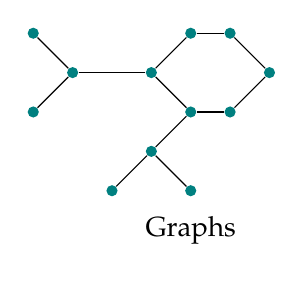
\begin{tikzpicture}[scale = .5,
                        dot/.style={circle, fill=teal, inner sep=.5mm}]
      \node[dot] (1) at (1,5) {};
      \node (8) at (6,3) {};
      \node[dot] (3) at (1,3) {};
      \node[dot] (2) at (2,4) {};
      \node[dot] (11) at (3,1) {};
      \node[dot] (4) at (4,4) {};
      \node[dot] (10) at (4,2) {};
      \node[dot] (5) at (5,5) {};
      \node[dot] (9) at (5,3) {};
      \node[dot] (12) at (5,1) {};
      \node[dot] (6) at (6,5) {};
      \node[dot] (8) at (6,3) {};
      \node[dot] (7) at (7,4) {};

      \foreach \x/\y in {1/2, 3/2, 2/4, 4/5, 4/9, 5/6, 6/7, 7/8, 8/9, 
                         9/10, 10/11, 10/12}
        \draw (\x) -- (\y);

      \node at (5,0) {Graphs};
    \end{tikzpicture}
    \hspace{3pc}  \pause
    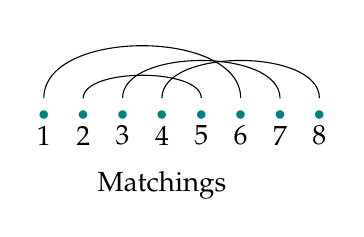
\begin{tikzpicture}[scale=.5]
      \node (1) at (1,0) {$\overset{ {\color{teal}{\bullet}} }{1}$};
      \node (2) at (2,0) {$\overset{ {\color{teal}{\bullet}} }{2}$};
      \node (3) at (3,0) {$\overset{ {\color{teal}{\bullet}} }{3}$};
      \node (4) at (4,0) {$\overset{ {\color{teal}{\bullet}} }{4}$};
      \node (5) at (5,0) {$\overset{ {\color{teal}{\bullet}} }{5}$};
      \node (6) at (6,0) {$\overset{ {\color{teal}{\bullet}} }{6}$};
      \node (7) at (7,0) {$\overset{ {\color{teal}{\bullet}} }{7}$};
      \node (8) at (8,0) {$\overset{ {\color{teal}{\bullet}} }{8}$};

      \draw (1) .. controls (1,2.5) and (6,2.5) .. (6);
      \draw (2) .. controls (2,1.5) and (5,1.5) .. (5);
      \draw (3) .. controls (3,2) and (7,2) .. (7);
      \draw (4) .. controls (4,2) and (8,2) .. (8);

      \node at (4,-1.5) {Matchings};
    \end{tikzpicture}

      \vspace{1pc}
    \pause
    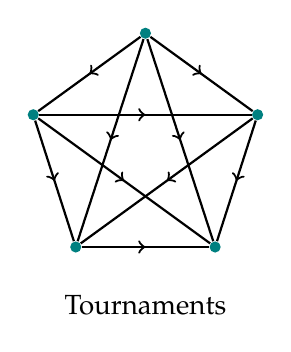
\begin{tikzpicture}[scale=.15,
                        dot/.style={circle, fill=teal, inner sep=.5mm}]
      \node[dot] (1) at (0,10) {};
      \node[dot] (2) at (9.5,3.1) {};
      \node[dot] (3) at (5.9,-8.1) {};
      \node[dot] (4) at (-5.9, -8.1) {};
      \node[dot] (5) at (-9.5, 3.1) {};
      
      \begin{scope}[thick,decoration={
          markings,
          mark=at position 0.5 with {\arrow{>}}}
          ] 
          \draw[postaction={decorate}] (1) -- (2);
          \draw[postaction={decorate}] (1) -- (3);
          \draw[postaction={decorate}] (1) -- (4);
          \draw[postaction={decorate}] (1) -- (5);

          \draw[postaction={decorate}] (2) -- (4);
          \draw[postaction={decorate}] (2) -- (3);
          \draw[postaction={decorate}] (5) -- (2);

          \draw[postaction={decorate}] (4) -- (3);
          \draw[postaction={decorate}] (5) -- (4);
          \draw[postaction={decorate}] (5) -- (3);



      \end{scope}

      \node at (0,-13) {Tournaments};
    \end{tikzpicture}
    \hspace{2pc}  \pause
    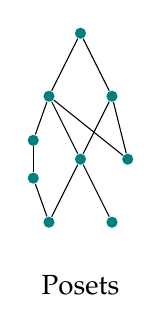
\begin{tikzpicture}[scale = .4,
                        dot/.style={circle, fill=teal, inner sep=.5mm}]
      \node[dot] (top1) at (0,4) {};
      \node[dot] (mid1) at (-1,2) {};
      \node[dot] (mid2) at (1,2) {};
      \node[dot] (bot11) at (-1.5,.6) {};
      \node[dot] (bot12) at (-1.5,-.6) {};
      \node[dot] (bot2) at (0,0) {};
      \node[dot] (bot3) at (1.5,0) {};
      \node[dot] (dwn1) at (-1,-2) {};
      \node[dot] (dwn2) at (1,-2) {};

      \draw (top1) -- (mid1);
      \draw (top1) -- (mid2);
      \draw (mid1) -- (bot11);
      \draw (bot11) -- (bot12);

      \draw (mid1) -- (bot2);
      \draw (mid1) -- (bot3);
      \draw (mid2) -- (bot2);
      \draw (mid2) -- (bot3);
      \draw (bot12) -- (dwn1);
      \draw (bot2) -- (dwn1);
      \draw (bot2) -- (dwn2);

      \node at (0, -4) {Posets};
    \end{tikzpicture}
    \hspace{2pc} \pause
    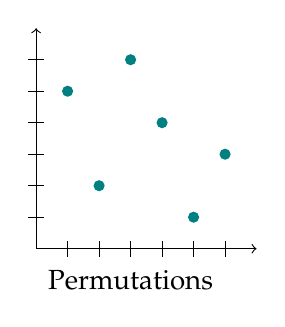
\begin{tikzpicture}[scale = .4,
                        dot/.style={circle, fill=teal, inner sep=.5mm}]
      \draw[->] (0,0) -- (7,0);
      \draw[->] (0,0) -- (0,7);
      \foreach \y [count = \x] in {5,2,6,4,1,3}{
        \node[dot] at (\x,\y) {};
        \draw (\x, -.25) -- (\x,.25);
        \draw (-.25, \x) -- (.25, \x);
      }
      \node at (3,-1) {Permutations};
    \end{tikzpicture}
    \end{center}
  \end{frame}


  \begin{frame}{Relational Structures}

    \begin{block}{Definition}
      A \emph{relational structure} consists of a \emph{ground set} together with
      a set of \emph{relations}, describable using first-order logic. 
    \end{block}
    \pause
    \begin{block}{Example}
      A graph is a ground set (vertices) together with a 2-relation (edges) which
      is symmetric and nonreflexive. 

      That is:
      $$ \mathcal{G} = (\mathcal{S}, \mathcal{R}) \text{, where }
      \mathcal{R} \subset \mathcal{S} \times \mathcal{S},$$
      with 
      $$ (x,y) \in \mathcal{R} \implies (y,x) \in \mathcal{R} \text{, and }
       (x,x) \notin \mathcal{R}\ \forall x \in \mathcal{S}.$$


    \end{block}

  \end{frame}
    

  \begin{frame}{Combinatorial Structures} 
    \setbeamercovered{transparent}
    \uncover<1>{
    \begin{center}
    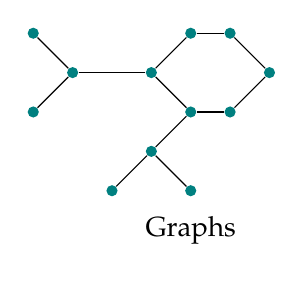
\begin{tikzpicture}[scale = .5,
                        dot/.style={circle, fill=teal, inner sep=.5mm}]
      \node[dot] (1) at (1,5) {};
      \node (8) at (6,3) {};
      \node[dot] (3) at (1,3) {};
      \node[dot] (2) at (2,4) {};
      \node[dot] (11) at (3,1) {};
      \node[dot] (4) at (4,4) {};
      \node[dot] (10) at (4,2) {};
      \node[dot] (5) at (5,5) {};
      \node[dot] (9) at (5,3) {};
      \node[dot] (12) at (5,1) {};
      \node[dot] (6) at (6,5) {};
      \node[dot] (8) at (6,3) {};
      \node[dot] (7) at (7,4) {};

      \foreach \x/\y in {1/2, 3/2, 2/4, 4/5, 4/9, 5/6, 6/7, 7/8, 8/9, 
                         9/10, 10/11, 10/12}
        \draw (\x) -- (\y);

      \node at (5,0) {Graphs};
    \end{tikzpicture}
    \hspace{3pc} 
    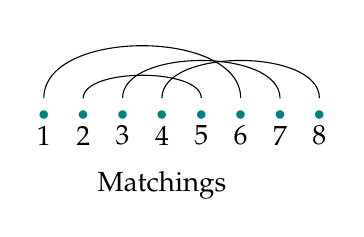
\begin{tikzpicture}[scale=.5]
      \node (1) at (1,0) {$\overset{ {\color{teal}{\bullet}} }{1}$};
      \node (2) at (2,0) {$\overset{ {\color{teal}{\bullet}} }{2}$};
      \node (3) at (3,0) {$\overset{ {\color{teal}{\bullet}} }{3}$};
      \node (4) at (4,0) {$\overset{ {\color{teal}{\bullet}} }{4}$};
      \node (5) at (5,0) {$\overset{ {\color{teal}{\bullet}} }{5}$};
      \node (6) at (6,0) {$\overset{ {\color{teal}{\bullet}} }{6}$};
      \node (7) at (7,0) {$\overset{ {\color{teal}{\bullet}} }{7}$};
      \node (8) at (8,0) {$\overset{ {\color{teal}{\bullet}} }{8}$};

      \draw (1) .. controls (1,2.5) and (6,2.5) .. (6);
      \draw (2) .. controls (2,1.5) and (5,1.5) .. (5);
      \draw (3) .. controls (3,2) and (7,2) .. (7);
      \draw (4) .. controls (4,2) and (8,2) .. (8);

      \node at (4,-1.5) {Matchings};
    \end{tikzpicture}

      \vspace{1pc}
    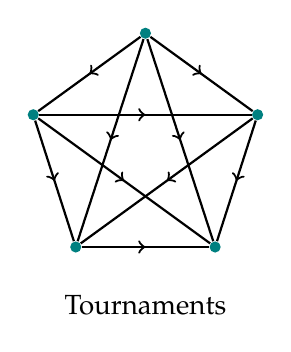
\begin{tikzpicture}[scale=.15,
                        dot/.style={circle, fill=teal, inner sep=.5mm}]
      \node[dot] (1) at (0,10) {};
      \node[dot] (2) at (9.5,3.1) {};
      \node[dot] (3) at (5.9,-8.1) {};
      \node[dot] (4) at (-5.9, -8.1) {};
      \node[dot] (5) at (-9.5, 3.1) {};
      
      \begin{scope}[thick,decoration={
          markings,
          mark=at position 0.5 with {\arrow{>}}}
          ] 
          \draw[postaction={decorate}] (1) -- (2);
          \draw[postaction={decorate}] (1) -- (3);
          \draw[postaction={decorate}] (1) -- (4);
          \draw[postaction={decorate}] (1) -- (5);

          \draw[postaction={decorate}] (2) -- (4);
          \draw[postaction={decorate}] (2) -- (3);
          \draw[postaction={decorate}] (5) -- (2);

          \draw[postaction={decorate}] (4) -- (3);
          \draw[postaction={decorate}] (5) -- (4);
          \draw[postaction={decorate}] (5) -- (3);



      \end{scope}

      \node at (0,-13) {Tournaments};
    \end{tikzpicture}
    \hspace{2pc} 
    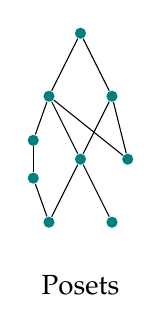
\begin{tikzpicture}[scale = .4,
                        dot/.style={circle, fill=teal, inner sep=.5mm}]
      \node[dot] (top1) at (0,4) {};
      \node[dot] (mid1) at (-1,2) {};
      \node[dot] (mid2) at (1,2) {};
      \node[dot] (bot11) at (-1.5,.6) {};
      \node[dot] (bot12) at (-1.5,-.6) {};
      \node[dot] (bot2) at (0,0) {};
      \node[dot] (bot3) at (1.5,0) {};
      \node[dot] (dwn1) at (-1,-2) {};
      \node[dot] (dwn2) at (1,-2) {};

      \draw (top1) -- (mid1);
      \draw (top1) -- (mid2);
      \draw (mid1) -- (bot11);
      \draw (bot11) -- (bot12);

      \draw (mid1) -- (bot2);
      \draw (mid1) -- (bot3);
      \draw (mid2) -- (bot2);
      \draw (mid2) -- (bot3);
      \draw (bot12) -- (dwn1);
      \draw (bot2) -- (dwn1);
      \draw (bot2) -- (dwn2);

      \node at (0, -4) {Posets};
    \end{tikzpicture}
    \hspace{2pc}
    }
    \uncover<1-2>{
    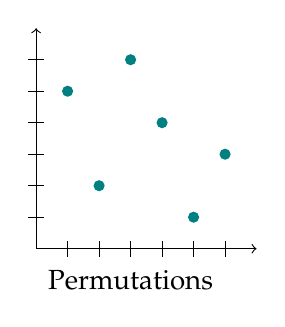
\begin{tikzpicture}[scale = .4,
                        dot/.style={circle, fill=teal, inner sep=.5mm}]
      \draw[->] (0,0) -- (7,0);
      \draw[->] (0,0) -- (0,7);
      \foreach \y [count = \x] in {5,2,6,4,1,3}{
        \node[dot] at (\x,\y) {};
        \draw (\x, -.25) -- (\x,.25);
        \draw (-.25, \x) -- (.25, \x);
      }
      \node at (3,-1) {Permutations};
    \end{tikzpicture}
    }
    \end{center}
  \end{frame}




% =========================================================================== %
  \section{Patterns in Data}
  \begin{frame}
    \centering
    \Large \color{teal} Patterns in Data \\{\large (and Permutations)}
  \end{frame}

  \begin{frame}{Random Data}
    \begin{center}
    \begin{tikzpicture}[scale=.885, only marks]
    \draw (-2.5,-2.5) -- (2.5,-2.5) -- (2.5,2.5) -- (-2.5,2.5) -- cycle;
    \draw plot[mark=*, mark size = .4mm] file {normaldata.txt};
    \end{tikzpicture}
    \end{center}
  \end{frame}

  \begin{frame} \frametitle{Permutations}
    \pause
    \begin{block}{Definition}
      An \emph{permutation of length $n$} is a bijection from the set $[n] = \{1,
      2, \dots n\}$ to itself. The \emph{one-line notation} for a permutation
      $\pi$ is 
      $$ \pi = \pi(1) \pi(2) \dots \pi(n). $$

      The set of all permutations of length $n$ is denoted $\S_n$. 
    \end{block}
    \pause
    \vspace{1pc}

    \begin{center}
    \begin{block}{Examples}
      \begin{itemize}
        \item The sequence $\pi = 5172643$ is a permutation of length $7$. 
        \pause
        \item The six permutations of length $3$ are 
          $$ \S_3 = \{123, 132, 213, 231, 312, 321\}. $$
      \end{itemize}
    \end{block}
    \end{center}
  \end{frame}

  \begin{frame} \frametitle{Plotting Permutations}
    \begin{block}{Definition}
      If $\pi$ is a permutation of length $n$, then the \emph{plot}
      of $\pi$ is the set of points 
      $$ \{ (1, \pi(1)), (2, \pi(2)), \cdots (n, \pi(n)) \} \subset \mathbb{R}^2 $$
    \end{block}

    \pause 
    \begin{center}
    \begin{tikzpicture}[scale = .5,
                        dot/.style={circle, fill=teal, inner sep=.5mm}]
      \draw[<->] (0,6) -- (0,0) -- (6,0);
      \foreach \y [count = \x] in {3,5,1,4,2}{
      % \node[dot, label=210:{{\tiny $(\x,\y)$}}] at (\x,\y) {};
        \node[dot] at (\x,\y) {};
        \draw (\x,-.25) -- (\x, .25);
        \draw (-.25, \x) -- (.25, \x);
      }
      \pause
      {\scriptsize
      \node[anchor=south west] at (3,1) {1};
      \pause
      \node[anchor=south west] at (5,2) {2};
      \pause
      \node[anchor=south west] at (1,3) {3};
      \pause
      \node[anchor=south west] at (4,4) {4};
      \pause
      \node[anchor=south west] at (2,5) {5};
      }
    \end{tikzpicture}
    \end{center}
    \uncover<2->{
    $$ \pi = 35142 $$
    }
  \end{frame}

  \begin{frame} \frametitle{Dots on a Plane} 
    \only<1->{
    \begin{block}{Definition} 
      Let $A$ and $B$ be two sets of $n$ points in $\R^2$, each with the property
      that no two points lie on the same horizontal or vertical line. \\
      Say that $A$ is \emph{order isomorphic} to $B$ (denoted $A \sim B$) if $A$
      can be transformed into $B$ by stretching, contracting, and translating the
      axes horizontally and vertically.
    \end{block}
    }
    
    \vspace{.5pc}

    \pause 

    \begin{block}{Example}
      \vspace{1pc}
      \begin{tikzpicture}[scale = .45,
                          dot/.style={circle, fill=teal, inner sep=.5mm}]
        \node[dot] at (1,3.5) {};
        \node[dot] at (1.3,4.5) {};
        \node[dot] at (3,.5) {};
        \node[dot] at (3.4,4) {};
        \node[dot] at (5,1) {};
        {\scriptsize
        \uncover<5->{\node[anchor=south west] at (3,.5) {1};}
        \uncover<6->{\node[anchor=south west] at (5,1) {2};}
        \uncover<7->{\node[anchor=south west] at (1,3.5) {3};}
        \uncover<8->{\node[anchor=south west] at (3.4,4) {4};}
        \uncover<9->{\node[anchor=south west] at (1.3,4.5) {5};}
        }
      \end{tikzpicture}
      \hspace{1pc}
      \raisebox{2.5pc}{$\sim$}
      \hspace{1pc}
      \begin{tikzpicture}[scale = .45,
                          dot/.style={circle, fill=teal, inner sep=.5mm}]
        \node[dot] at (1,2) {};
        \node[dot] at (2.5,5) {};
        \node[dot] at (3,1) {};
        \node[dot] at (3.5,4) {};
        \node[dot] at (5,1.5) {};
        {\scriptsize
        \uncover<5->{\node[anchor=south west] at (3,1) {1};}
        \uncover<6->{\node[anchor=south west] at (5,1.5) {2};}
        \uncover<7->{\node[anchor=south west] at (1,2) {3};}
        \uncover<8->{\node[anchor=south west] at (3.5,4) {4};}
        \uncover<9->{\node[anchor=south west] at (2.5,5) {5};}
        }
      \end{tikzpicture}
      \hspace{1pc}
      \pause
      \raisebox{2.5pc}{$\sim$}
      \hspace{1pc}
      \begin{tikzpicture}[scale = .45,
                          dot/.style={circle, fill=teal, inner sep=.5mm}]
        \foreach \y [count = \x] in {3,5,1,4,2}
        \node[dot] at (\x,\y) {};
        {\scriptsize
        \uncover<5->{\node[anchor=south west] at (3,1) {1};}
        \uncover<6->{\node[anchor=south west] at (5,2) {2};}
        \uncover<7->{\node[anchor=south west] at (1,3) {3};}
        \uncover<8->{\node[anchor=south west] at (4,4) {4};}
        \uncover<9->{\node[anchor=south west] at (2,5) {5};}
        }
      \end{tikzpicture}

      \pause
      \vspace{1pc}
      { \hfill $\pi = 35142$ \hspace{2pc}}
    \end{block}
  \end{frame}

  \begin{frame}{Permutation Symmetries} \pause
    \begin{block}{Definition}
      For a permutation $\pi = \pi_1 \pi_2 \dots \pi_n$ , the reverse, the
      complement, and the inverse of $\pi$ are denoted $\pi^r$, $\pi^c$, and
      $\pi^{-1}$, and defined as follows: 
      $$ (\pi^r)_i = \pi_{n+1 - i}, \quad (\pi^c)_i = n + 1 - \pi_i, \text{ and} $$
      $$ (\pi^{-1})_{\pi_j} = j.$$
    \end{block}
    \pause
    \begin{center}
      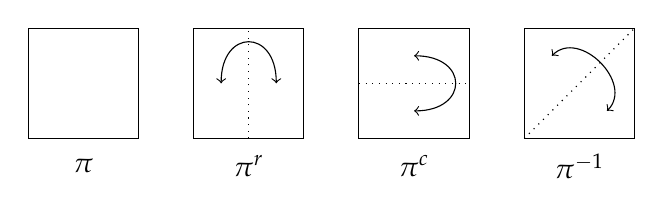
\begin{tikzpicture}[scale=.35]
      \draw (0,0) rectangle (4,4);
      \node at (2,-1) {$\pi$};

      \pause
      \draw (6,0) rectangle (10,4);
      \node at (8,-1) {$\pi^r$};
      \draw[dotted] (8,0) -- (8,4);
      \draw[<->] (7,2) .. controls (7,4) and (9,4) .. (9,2);
        
      \pause
      \draw (12,0) rectangle (16,4);
      \node at (14,-1) {$\pi^c$};
      \draw[dotted] (12,2) -- (16,2);
      \draw[<->] (14,1) .. controls (16,1) and (16,3) .. (14,3);

      \pause
      \draw (18,0) rectangle (22,4);
      \node at (20,-1) {$\pi^{-1}$};
      \draw[dotted] (18,0) -- (22,4);
      \draw[<->] (19,3) .. controls (20,4) and (22,2) .. (21,1);

      \end{tikzpicture}
    \end{center}
  \end{frame}



  \begin{frame}{Random Data}
    \begin{center}
      \begin{tikzpicture}[scale=.885, only marks]
      \draw (-2.5,-2.5) -- (2.5,-2.5) -- (2.5,2.5) -- (-2.5,2.5) -- cycle;
      \draw plot[mark=*, mark size = .4mm] file {normaldata.txt};
      \end{tikzpicture}
      % \begin{tikzpicture}[scale=4, only marks]
      % \draw (-0.05,-0.05) -- (1.05,-0.05) -- (1.05,1.05) -- (-0.05,1.05) -- cycle;
      % \draw plot[mark=*, mark size = .1mm] file {normaldata.txt};
      % \end{tikzpicture}
      \pause
      \hspace{4pt}
      \raisebox{5pc}{$\sim$}
      \hspace{4pt}
      \begin{tikzpicture}[scale=4, only marks]
      \draw (-0.05,-0.05) -- (1.05,-0.05) -- (1.05,1.05) -- (-0.05,1.05) -- cycle;
      \draw plot[mark=*, mark size = .1mm] file {organizeddata.txt};
      \end{tikzpicture}
    \end{center}
    \pause
    { \scriptsize
    $$ \begin{aligned}\pi &= 
        61\ 84\ 31\ 35\ 39\ 28\ 9\ 54\ 6\ 4\ 74\ 71\ 68\ 85\ 98\ 38\ 97\ 45\ 12\
        27\ 57\ 89\ 30\ 5\ 55\ 11\ 58\ \\
        &13\ 42\ 32\ 14\ 53\ 2\ 51\ 20\ 56\ 80\ 10\ 43\ 95\ 17\ 50\ 8\ 16\ 15\ 70\
        63\ 81\ 64\ 24\ 52\ 76\ 47\ \\
        &7\ 60\ 49\ 82\ 1\ 25\ 75\ 40\ 34\ 83\ 90\ 46\ 100\ 69\ 65\ 93\ 86\ 22\
        96\ 21\ 92\ 3\ 79\ 29\ 41\  \\
        &44\ 66\ 94\ 59\ 87\ 37\ 73\ 36\ 72\ 67\ 78\ 19\ 33\ 88\ 62\ 99\ 23\ 91\
        26\ 48\ 18\ 77
    \end{aligned}$$
    }
  \end{frame}

  \begin{frame} \frametitle{Permutation Patterns} \pause
    \begin{block}{Definition}
      Let $\pi = \pi(1) \pi(2) \cdots \pi(n)$ and 
      $\sg = \sg(1) \sg(2) \cdots \sg(k)$ be two permutations.
      $\pi$ \emph{contains $\sg$ as a pattern} (written $\sg \prec
      \pi$) if there is some subsequence $\pi(i_1) \pi(i_2) \ldots \pi(i_k)$
      which is order isomorphic to the entries of $\sg$ (i.e.,
      $\pi(i_j) < \pi(i_k)$ if and only if $\sg(j) < \sg(k)$).  
    \end{block}
    \pause 

    \vspace{1pc}

    \begin{center}
    \begin{tikzpicture}[scale = .5,
                        dot/.style={circle, fill=teal, inner sep=.5mm}]
      \node[dot] at (1,2) {};
      \node[dot] at (2,1) {};
      \node[dot] at (3,3) {};
      \node[] at (1,0) {};
    \end{tikzpicture}
    %
      \hspace{1pc}
      \raisebox{2pc}{$\prec$}
      \hspace{1pc}
    %
    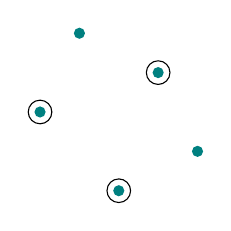
\begin{tikzpicture}[scale = .5,
                        dot/.style={circle, fill=teal, inner sep=.5mm}]
      \foreach \y [count = \x] in {3,5,1,4,2}
      \node[dot] at (\x,\y) {};
      \uncover<4>{
        \draw (1,3) circle (3mm);
        \draw (3,1) circle (3mm);
        \draw (4,4) circle (3mm);
      }
        
    \end{tikzpicture}
    \end{center}

    \vspace{1pc}

    $$ 213 \qquad \prec \qquad 
      \only<4>{\mathbf}35\only<4>{\mathbf}1\only<4>{\mathbf}42 $$
  \end{frame}

  \begin{frame} \frametitle{Permutation Patters}
    \begin{block}{Example}
      The pattern $12$ is contained in all permutations \emph{except} for the
      decreasing ones: 
      $$ 12 \not \prec n \dots 3 2 1 .$$ 
    \end{block}
    
    \pause 

    \begin{block}{Definition}
      If a permutation $\pi$ does not contain a pattern $\sg$, we say that $\pi$
      \emph{avoids} $\sg$. The set of all permutations which avoid a given
      pattern (or set of patterns) $\sg$ is denoted 
      $$ \Av(\sg).$$
    \end{block}
  \end{frame}


  \begin{frame} \frametitle{Permutation Classes} \pause
    \begin{block}{Definition}
      A \emph{permutation class} is a set $\C$ of permutations for which, if $\pi
      \in \C$ and $\sg \prec \pi$, then $\sg \in \C$. Let $\C_n$ denote the
      set of permutations of length $n$ in $\C$. 
    \end{block}

    \pause 
    \begin{block}{Example}
      $\Av(\sg)$ is a permutation class for any pattern (or set of patterns)
      $\sg$. 
    \end{block}

    \pause

    \begin{block}{Theorem (Marcus and Tardos, 2004)}
      Every proper permutation class has a finite exponential growth rate. That
      is, for any proper class $\C$, there exists a real number $s$ such that $$
      \limsup_{n \ra \infty} \sqrt[n]{|\C_n|} = s. $$

      This number $s$ is the \emph{growth rate} of the class. 
    \end{block}
  \end{frame}

  \newgeometry{margin=0mm}
  \begin{frame} \frametitle{\hspace{28pt}Permutation Classes - Growth Rates} 
    \begin{center}
      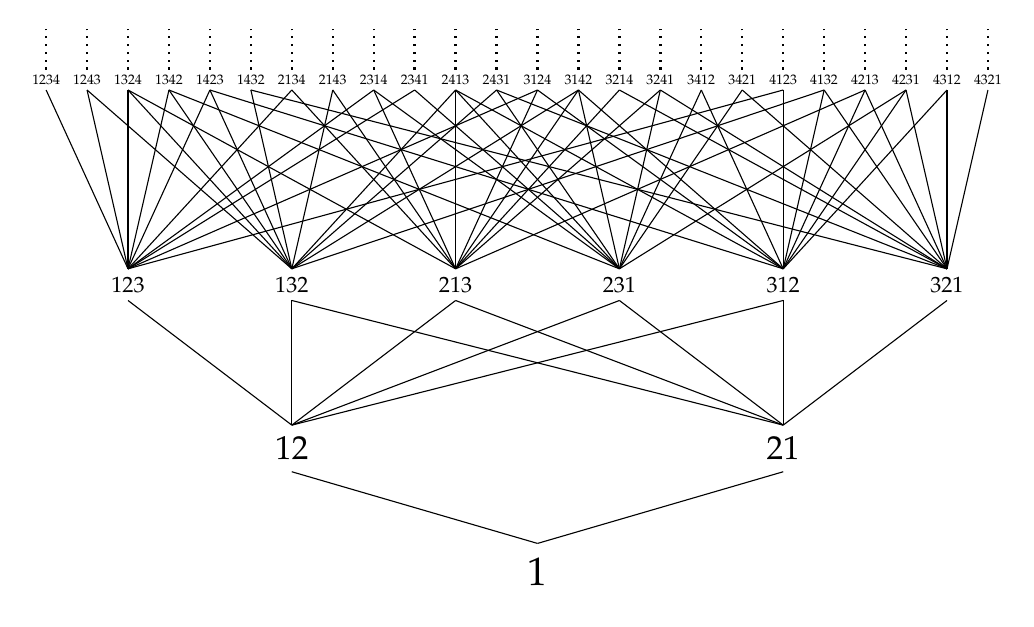
\begin{tikzpicture}[
      every node/.style={},
      scale=.52]
        {\Large
        \node (1) at (12,0) {1};
        }


        {\large
        \node (12) at (6,3) {12};
        \node (21) at (18,3) {21};
        }


        \draw (12.south)-- (1.north);
        \draw (21.south) -- (1.north);


        {\footnotesize
        \node (123) at (2 ,7) {123};
        \node (132) at (6 ,7) {132};
        \node (213) at (10,7) {213};
        \node (231) at (14,7) {231};
        \node (312) at (18,7) {312};
        \node (321) at (22,7) {321};
        }

        \draw (123.south) -- (12.north);
        \draw (132.south) -- (12.north);
        \draw (213.south) -- (12.north);
        \draw (231.south) -- (12.north);
        \draw (312.south) -- (12.north);
        
        \draw (132.south) -- (21.north);
        \draw (213.south) -- (21.north);
        \draw (231.south) -- (21.north);
        \draw (312.south) -- (21.north);
        \draw (321.south) -- (21.north);

        {\tiny
        \node (1234) at (0 ,12) {1234};
        \node (1243) at (1 ,12) {1243};
        \node (1324) at (2 ,12) {1324};
        \node (1342) at (3 ,12) {1342};
        \node (1423) at (4 ,12) {1423};
        \node (1432) at (5 ,12) {1432};

        \node (2134) at (6 ,12) {2134};
        \node (2143) at (7 ,12) {2143};
        \node (2314) at (8 ,12) {2314};
        \node (2341) at (9 ,12) {2341};
        \node (2413) at (10,12) {2413};
        \node (2431) at (11,12) {2431};

        \node (3124) at (12,12) {3124};
        \node (3142) at (13,12) {3142};
        \node (3214) at (14,12) {3214};
        \node (3241) at (15,12) {3241};
        \node (3412) at (16,12) {3412};
        \node (3421) at (17,12) {3421};

        \node (4123) at (18,12) {4123};
        \node (4132) at (19,12) {4132};
        \node (4213) at (20,12) {4213};
        \node (4231) at (21,12) {4231};
        \node (4312) at (22,12) {4312};
        \node (4321) at (23,12) {4321};
        }

        % 123
        \foreach \p in {1234, 1243, 1324, 1342, 1423, 2134, 2314, 2341, 3124, 4123}
          \draw (\p.south) -- (123.north);
        % 132
        \foreach \p in {1243, 1324, 1342, 1423, 1432, 2143, 2413, 2431, 3142, 4132}
          \draw (\p.south) -- (132.north);
        % 213
        \foreach \p in {1324, 2134, 2143, 2314, 2413, 3124, 3142, 3214, 3241, 4213}
          \draw (\p.south) -- (213.north);
        % 231
        \foreach \p in {1342, 2314, 2341, 2413, 2431, 3142, 3241, 3412, 3421, 4231}
          \draw (\p.south) -- (231.north);
        % 312
        \foreach \p in {1423, 2413, 3124, 3142, 3412, 4123, 4132, 4213, 4231, 4312}
          \draw (\p.south) -- (312.north);
        % 321
        \foreach \p in {4321, 3421, 4231, 2431, 3241, 4312, 4132, 1432, 4213, 3214}
          \draw (\p.south) -- (321.north);

        \foreach \p in {1234, 1243, 1324, 1342, 1423, 1432,
                        2134, 2143, 2314, 2341, 2413, 2431,
                        3124, 3142, 3214, 3241, 3412, 3421,
                        4123, 4132, 4213, 4231, 4312, 4321}
          \draw[dotted, line width=.3mm] (\p.north) -- ++(0,1);

      \end{tikzpicture}
    \end{center}
  \end{frame}



  % =========================================================================== %
  \begin{frame} \frametitle{\hspace{28pt}Permutation Classes - Growth Rates} 
    \begin{center}
      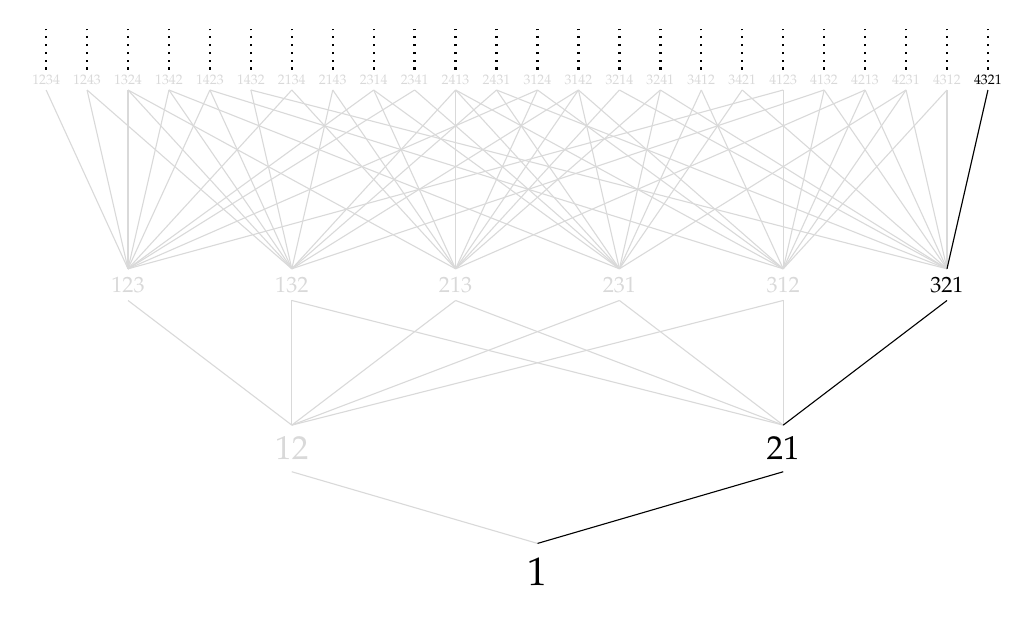
\begin{tikzpicture}[
      every node/.style={},
      scale=.52]
        {\Large
        \node (1) at (12,0) {1};
        }


        {\large
        \node (12) at (6,3) {\color{lg}{12}};
        \node (21) at (18,3) {21};
        }


        \draw[color=lg] (12.south)-- (1.north);
        \draw (21.south) -- (1.north);


        {\footnotesize
        \node (123) at (2 ,7) {\color{lg}{123}};
        \node (132) at (6 ,7) {\color{lg}{132}};
        \node (213) at (10,7) {\color{lg}{213}};
        \node (231) at (14,7) {\color{lg}{231}};
        \node (312) at (18,7) {\color{lg}{312}};
        \node (321) at (22,7) {321};
        }

        \draw[color=lg] (123.south) -- (12.north);
        \draw[color=lg] (132.south) -- (12.north);
        \draw[color=lg] (213.south) -- (12.north);
        \draw[color=lg] (231.south) -- (12.north);
        \draw[color=lg] (312.south) -- (12.north);
        
        \draw[color=lg] (132.south) -- (21.north);
        \draw[color=lg] (213.south) -- (21.north);
        \draw[color=lg] (231.south) -- (21.north);
        \draw[color=lg] (312.south) -- (21.north);
        \draw (321.south) -- (21.north);

        {\tiny
        \node (1234) at (0 ,12) {\color{lg}{1234}};
        \node (1243) at (1 ,12) {\color{lg}{1243}};
        \node (1324) at (2 ,12) {\color{lg}{1324}};
        \node (1342) at (3 ,12) {\color{lg}{1342}};
        \node (1423) at (4 ,12) {\color{lg}{1423}};
        \node (1432) at (5 ,12) {\color{lg}{1432}};

        \node (2134) at (6 ,12) {\color{lg}{2134}};
        \node (2143) at (7 ,12) {\color{lg}{2143}};
        \node (2314) at (8 ,12) {\color{lg}{2314}};
        \node (2341) at (9 ,12) {\color{lg}{2341}};
        \node (2413) at (10,12) {\color{lg}{2413}};
        \node (2431) at (11,12) {\color{lg}{2431}};

        \node (3124) at (12,12) {\color{lg}{3124}};
        \node (3142) at (13,12) {\color{lg}{3142}};
        \node (3214) at (14,12) {\color{lg}{3214}};
        \node (3241) at (15,12) {\color{lg}{3241}};
        \node (3412) at (16,12) {\color{lg}{3412}};
        \node (3421) at (17,12) {\color{lg}{3421}};

        \node (4123) at (18,12) {\color{lg}{4123}};
        \node (4132) at (19,12) {\color{lg}{4132}};
        \node (4213) at (20,12) {\color{lg}{4213}};
        \node (4231) at (21,12) {\color{lg}{4231}};
        \node (4312) at (22,12) {\color{lg}{4312}};
        \node (4321) at (23,12) {4321};
        }

        % 123
        \foreach \p in {1234, 1243, 1324, 1342, 1423, 2134, 2314, 2341, 3124, 4123}
          \draw[color=lg] (\p.south) -- (123.north);
        % 132
        \foreach \p in {1243, 1324, 1342, 1423, 1432, 2143, 2413, 2431, 3142, 4132}
          \draw[color=lg] (\p.south) -- (132.north);
        % 213
        \foreach \p in {1324, 2134, 2143, 2314, 2413, 3124, 3142, 3214, 3241, 4213}
          \draw[color=lg] (\p.south) -- (213.north);
        % 231
        \foreach \p in {1342, 2314, 2341, 2413, 2431, 3142, 3241, 3412, 3421, 4231}
          \draw[color=lg] (\p.south) -- (231.north);
        % 312
        \foreach \p in {1423, 2413, 3124, 3142, 3412, 4123, 4132, 4213, 4231, 4312}
          \draw[color=lg] (\p.south) -- (312.north);
        % 321
        \foreach \p in {4321, 3421, 4231, 2431, 3241, 4312, 4132, 1432, 4213, 3214}
          \draw[color=lg] (\p.south) -- (321.north);
        \draw (321.north) -- (4321.south);

        \foreach \p in {1234, 1243, 1324, 1342, 1423, 1432,
                        2134, 2143, 2314, 2341, 2413, 2431,
                        3124, 3142, 3214, 3241, 3412, 3421,
                        4123, 4132, 4213, 4231, 4312, 4321}
          \draw[dotted, line width=.3mm] (\p.north) -- ++(0,1);

      \end{tikzpicture}
    \end{center}
  \end{frame}

  % =========================================================================== %
  \begin{frame} \frametitle{\hspace{28pt}Permutation Classes - Growth Rates} 
    \begin{center}
      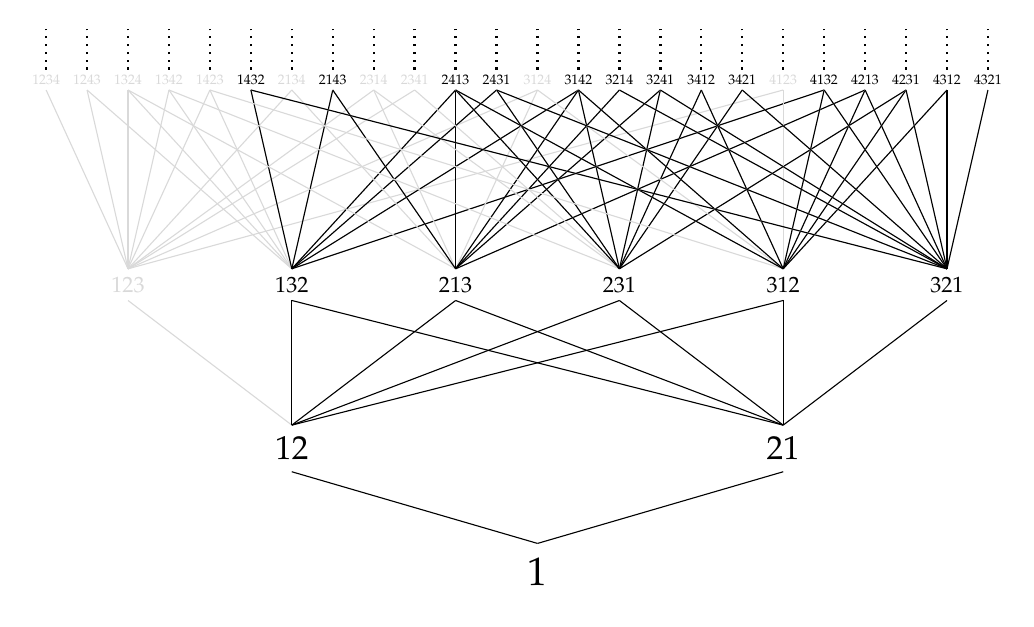
\begin{tikzpicture}[
      every node/.style={},
      scale=.52]
        {\Large
        \node (1) at (12,0) {1};
        }


        {\large
        \node (12) at (6,3) {12};
        \node (21) at (18,3) {21};
        }


        \draw (12.south)-- (1.north);
        \draw (21.south) -- (1.north);


        {\footnotesize
        \node (123) at (2 ,7) {\color{lg}{123}};
        \node (132) at (6 ,7) {132};
        \node (213) at (10,7) {213};
        \node (231) at (14,7) {231};
        \node (312) at (18,7) {312};
        \node (321) at (22,7) {321};
        }

        \draw[color=lg] (123.south) -- (12.north);
        \draw (132.south) -- (12.north);
        \draw (213.south) -- (12.north);
        \draw (231.south) -- (12.north);
        \draw (312.south) -- (12.north);
        
        \draw (132.south) -- (21.north);
        \draw (213.south) -- (21.north);
        \draw (231.south) -- (21.north);
        \draw (312.south) -- (21.north);
        \draw (321.south) -- (21.north);

        {\tiny
        \node (1234) at (0 ,12) {\color{lg}{1234}};
        \node (1243) at (1 ,12) {\color{lg}{1243}};
        \node (1324) at (2 ,12) {\color{lg}{1324}};
        \node (1342) at (3 ,12) {\color{lg}{1342}};
        \node (1423) at (4 ,12) {\color{lg}{1423}};
        \node (1432) at (5 ,12) {1432};

        \node (2134) at (6 ,12) {\color{lg}{2134}};
        \node (2143) at (7 ,12) {2143};
        \node (2314) at (8 ,12) {\color{lg}{2314}};
        \node (2341) at (9 ,12) {\color{lg}{2341}};
        \node (2413) at (10,12) {2413};
        \node (2431) at (11,12) {2431};

        \node (3124) at (12,12) {\color{lg}{3124}};
        \node (3142) at (13,12) {3142};
        \node (3214) at (14,12) {3214};
        \node (3241) at (15,12) {3241};
        \node (3412) at (16,12) {3412};
        \node (3421) at (17,12) {3421};

        \node (4123) at (18,12) {\color{lg}{4123}};
        \node (4132) at (19,12) {4132};
        \node (4213) at (20,12) {4213};
        \node (4231) at (21,12) {4231};
        \node (4312) at (22,12) {4312};
        \node (4321) at (23,12) {4321};
        }

        % 123
        \foreach \p in {1234, 1243, 1324, 1342, 1423, 2134, 2314, 2341, 3124, 4123}
          \draw[color=lg] (\p.south) -- (123.north);
        % 132
        \foreach \p in {1243, 1324, 1342, 1423, 1432, 2143, 2413, 2431, 3142, 4132}
          \draw[color=lg] (\p.south) -- (132.north);

        \foreach \p in {1432, 2143, 2413, 2431, 3142, 4132}
          \draw[] (\p.south) -- (132.north);

        % 213
        \foreach \p in {1324, 2134, 2143, 2314, 2413, 3124, 3142, 3214, 3241, 4213}
          \draw[color=lg] (\p.south) -- (213.north);

        \foreach \p in {2143, 2413, 3142, 3214, 3241, 4213}
          \draw[] (\p.south) -- (213.north);

        % 231
        \foreach \p in {1342, 2314, 2341, 2413, 2431, 3142, 3241, 3412, 3421, 4231}
          \draw[color=lg] (\p.south) -- (231.north);

        \foreach \p in {2413, 2431, 3142, 3241, 3412, 3421, 4231}
          \draw[] (\p.south) -- (231.north);

        % 312
        \foreach \p in {1423, 2413, 3124, 3142, 3412, 4123, 4132, 4213, 4231, 4312}
          \draw[color=lg] (\p.south) -- (312.north);

        \foreach \p in {2413, 3142, 3412, 4132, 4213, 4231, 4312}
          \draw[] (\p.south) -- (312.north);

        % 321
        \foreach \p in {4321, 3421, 4231, 2431, 3241, 4312, 4132, 1432, 4213, 3214}
          \draw[color=lg] (\p.south) -- (321.north);

        \foreach \p in {4321, 3421, 4231, 2431, 3241, 4312, 4132, 1432, 4213, 3214}
          \draw[] (\p.south) -- (321.north);


        \foreach \p in {1234, 1243, 1324, 1342, 1423, 1432,
                        2134, 2143, 2314, 2341, 2413, 2431,
                        3124, 3142, 3214, 3241, 3412, 3421,
                        4123, 4132, 4213, 4231, 4312, 4321}
          \draw[dotted, line width=.3mm] (\p.north) -- ++(0,1);

      \end{tikzpicture}
    \end{center}
  \end{frame}



  % =========================================================================== %
  \begin{frame} \frametitle{\hspace{28pt}Permutation Classes - Growth Rates} 
    \begin{center}
      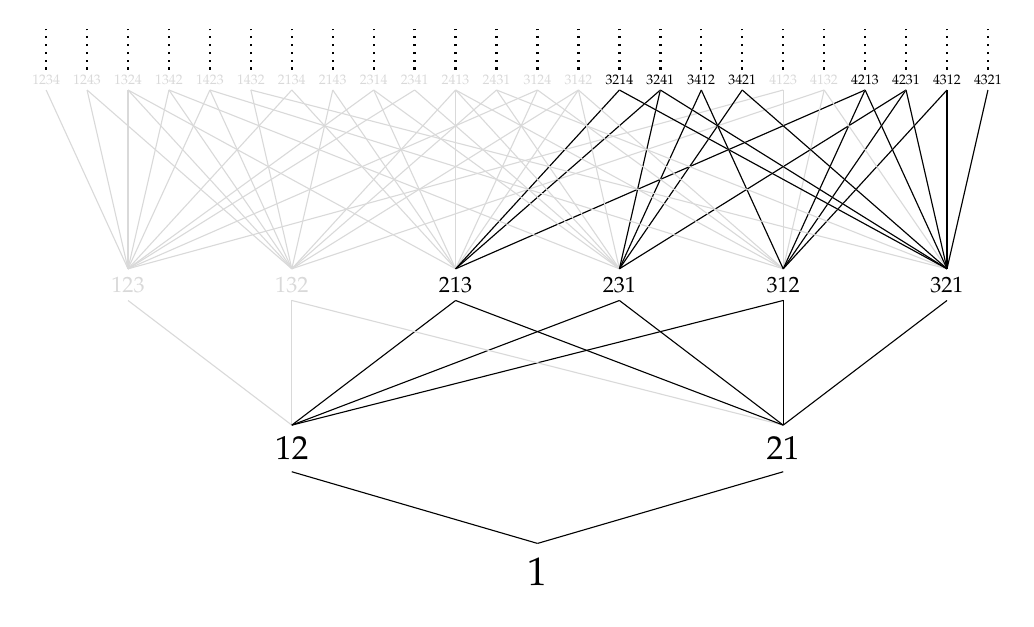
\begin{tikzpicture}[
      every node/.style={},
      scale=.52]
        {\Large
        \node (1) at (12,0) {1};
        }


        {\large
        \node (12) at (6,3) {12};
        \node (21) at (18,3) {21};
        }


        \draw (12.south)-- (1.north);
        \draw (21.south) -- (1.north);


        {\footnotesize
        \node (123) at (2 ,7) {\color{lg}{123}};
        \node (132) at (6 ,7) {\color{lg}{132}};
        \node (213) at (10,7) {213};
        \node (231) at (14,7) {231};
        \node (312) at (18,7) {312};
        \node (321) at (22,7) {321};
        }

        \draw[color=lg] (123.south) -- (12.north);
        \draw[color=lg] (132.south) -- (12.north);
        \draw (213.south) -- (12.north);
        \draw (231.south) -- (12.north);
        \draw (312.south) -- (12.north);
        
        \draw[color=lg] (132.south) -- (21.north);
        \draw (213.south) -- (21.north);
        \draw (231.south) -- (21.north);
        \draw (312.south) -- (21.north);
        \draw (321.south) -- (21.north);

        {\tiny
        \node (1234) at (0 ,12) {\color{lg}{1234}};
        \node (1243) at (1 ,12) {\color{lg}{1243}};
        \node (1324) at (2 ,12) {\color{lg}{1324}};
        \node (1342) at (3 ,12) {\color{lg}{1342}};
        \node (1423) at (4 ,12) {\color{lg}{1423}};
        \node (1432) at (5 ,12) {\color{lg}{1432}};

        \node (2134) at (6 ,12) {\color{lg}{2134}};
        \node (2143) at (7 ,12) {\color{lg}{2143}};
        \node (2314) at (8 ,12) {\color{lg}{2314}};
        \node (2341) at (9 ,12) {\color{lg}{2341}};
        \node (2413) at (10,12) {\color{lg}{2413}};
        \node (2431) at (11,12) {\color{lg}{2431}};

        \node (3124) at (12,12) {\color{lg}{3124}};
        \node (3142) at (13,12) {\color{lg}{3142}};
        \node (3214) at (14,12) {3214};
        \node (3241) at (15,12) {3241};
        \node (3412) at (16,12) {3412};
        \node (3421) at (17,12) {3421};

        \node (4123) at (18,12) {\color{lg}{4123}};
        \node (4132) at (19,12) {\color{lg}{4132}};
        \node (4213) at (20,12) {4213};
        \node (4231) at (21,12) {4231};
        \node (4312) at (22,12) {4312};
        \node (4321) at (23,12) {4321};
        }


        % 123
        \foreach \p in {1234, 1243, 1324, 1342, 1423, 2134, 2314, 2341, 3124, 4123}
          \draw[color=lg] (\p.south) -- (123.north);
        % 132
        \foreach \p in {1243, 1324, 1342, 1423, 1432, 2143, 2413, 2431, 3142, 4132}
          \draw[color=lg] (\p.south) -- (132.north);

        % 213
        \foreach \p in {1324, 2134, 2143, 2314, 2413, 3124, 3142, 3214, 3241, 4213}
          \draw[color=lg] (\p.south) -- (213.north);

        \foreach \p in {3214, 3241, 4213}
          \draw[] (\p.south) -- (213.north);

        % 231
        \foreach \p in {1342, 2314, 2341, 2413, 2431, 3142, 3241, 3412, 3421, 4231}
          \draw[color=lg] (\p.south) -- (231.north);

        \foreach \p in {3241, 3412, 3421, 4231}
          \draw[] (\p.south) -- (231.north);

        % 312
        \foreach \p in {1423, 2413, 3124, 3142, 3412, 4123, 4132, 4213, 4231, 4312}
          \draw[color=lg] (\p.south) -- (312.north);

        \foreach \p in {3412, 4213, 4231, 4312}
          \draw[] (\p.south) -- (312.north);

        % 321
        \foreach \p in {4321, 3421, 4231, 2431, 3241, 4312, 4132, 1432, 4213, 3214}
          \draw[color=lg] (\p.south) -- (321.north);

        \foreach \p in {4321, 3421, 4231, 3241, 4312, 4213, 3214}
          \draw[] (\p.south) -- (321.north);



        \foreach \p in {1234, 1243, 1324, 1342, 1423, 1432,
                        2134, 2143, 2314, 2341, 2413, 2431,
                        3124, 3142, 3214, 3241, 3412, 3421,
                        4123, 4132, 4213, 4231, 4312, 4321}
          \draw[dotted, line width=.3mm] (\p.north) -- ++(0,1);

      \end{tikzpicture}
    \end{center}
  \end{frame}
  \restoregeometry
  \newgeometry{top=0mm,left=2pc, right=1pc}

  \begin{frame}\frametitle{The Class $\Av(132)$}
    \begin{block}{Definition}
      Let $c_n$ be the number of permutations of length $n$ which \emph{avoid}
      the pattern $132$, and $ C(x) = \sum_{n \geq 0} c_n x^n$.
    \end{block}

    \pause     

    \begin{block}{Question}
      What does a $132$-avoiding permutation look like?
    \end{block}

    \pause

    \begin{center}
    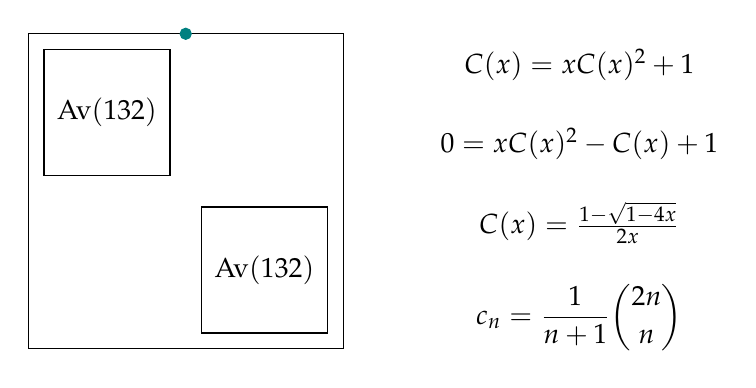
\begin{tikzpicture}[%
      scale=.2,
      filled/.style={circle, fill=teal, draw=teal, inner sep=.5mm}]

      \draw (0,0) -- (0,20) -- (20,20) -- (20, 0) -- cycle;
      \pause 
      \node[filled] at (10,20) {};
      \pause 

      \draw (1,11) -- (9,11) -- (9,19) -- (1,19) -- cycle;
      \draw (11, 1) -- (19,1) -- (19, 9) -- (11,9) -- cycle; 
      \pause

      \node at (5,15) {$\Av(132)$};
      \node at (15,5) {$\Av(132)$};

      \pause 
      \node at (35,18) {$C(x) = x C(x)^2 + 1$};
      \pause
      \node at (35,13) {$0 = x C(x)^2 - C(x) + 1$};
      \pause
      \node at (35, 8) {$C(x) = \frac{1 - \sqrt{1 - 4x}}{2x}$};
      \pause
      \node at (35, 2) {$ \displaystyle c_n = \frac{1}{n+1} \binom{2n}{n}$};

    \end{tikzpicture}
    \end{center}
  \end{frame} 


  \begin{frame}\frametitle{The Class $\Av(123)$} \pause
    \begin{block}{Question}
      What does a $123$-avoiding permutation look like?
    \end{block}
    \begin{center}
    \begin{tikzpicture}[scale=.18]
      \draw (0,0) -- (0,20) -- (20,20) -- (20, 0) -- cycle;
      \pause
      \draw (6,18) -- (18, 6);
      \draw (2,14) -- (14, 2);
      \node at (0,-3) {};
    \end{tikzpicture}
    \hspace{1pc}
    \pause
    \uncover<3->{
    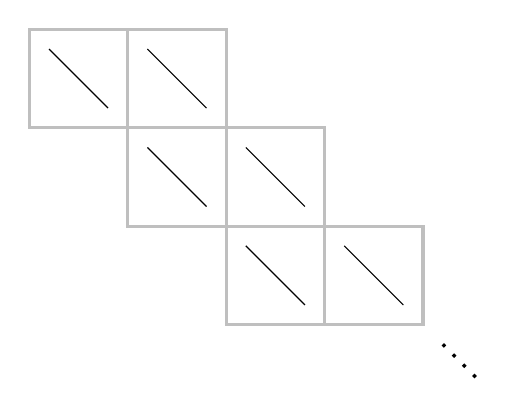
\begin{tikzpicture}[scale=.25, yscale=1]
      % draw the outer boxes, using a loop
      \foreach \x/\y in {0/10, 5/10, 5/5, 10/5,10/0, 15/0 }{
        \draw[very thick, color=lightgray] (\x, \y) rectangle (\x + 5, \y + 5);
        \draw (\x+1, \y+4) -- (\x+4,\y+1);
        \pause
      }
      \draw[very thick, loosely dotted] (21,-1) -- (23,-3);
      % closed dots
    \end{tikzpicture}
    }
    \end{center}
  \end{frame}

  \begin{frame} \frametitle{Av(132) and Av(123)}

    \begin{center}
      \begin{tikzpicture}[scale=.5]
      \only<1,3>{%
        \draw (1,1) -- (1,9) -- (9,9) -- (9,1) -- cycle;
        \foreach \y [count = \x] in {7,4,3,5,2,6,8,1}{
          \draw[fill = black] (\x+.5,\y+.5) circle (2mm);
        }
        \foreach \i in {1, ...,9}{
          \draw[dotted] (\i,1) -- (\i,9);
          \draw[dotted] (1,\i) -- (9,\i);
        }
        \node at (5,-1) {$\Av(132)$};
      }
      \only<2>{%
        \draw (1,1) -- (1,9) -- (9,9) -- (9,1) -- cycle;
        \foreach \y [count = \x] in {7,4,3,5,2,6,8,1}{
          \draw[fill = black] (\x+.5,\y+.5) circle (2mm);
        }
        \foreach \i in {1, ...,9}{
          \draw[dotted] (\i,1) -- (\i,9);
          \draw[dotted] (1,\i) -- (9,\i);
        }
        \draw[very thick] (1,2) rectangle (7,8);
        \draw[very thick] (8,1) rectangle (9,2);
        \node at (5,-1) {$\Av(132)$};
      }
      \only<4,7>{%
        \draw (1,1) -- (1,9) -- (9,9) -- (9,1) -- cycle;
        \foreach \y [count = \x] in {7,4,3,5,2,6,8,1}{
          \draw[fill = black] (\x+.5,\y+.5) circle (2mm);
        }
        \foreach \i in {1, ...,9}{
          \draw[dotted] (\i,1) -- (\i,9);
          \draw[dotted] (1,\i) -- (9,\i);
        }
        \draw[very thick] (1,9) --++ (0,-2) --++ (1,0) --++ (0,-3)
                          --++ (1,0) --++(0,-1) --++(2,0) 
                          --++ (0,-1) --++ (3,0) --++(0,-1) 
                          --++ (1,0);
        \node at (5,-1) {$\Av(132)$};
      }
      \only<5>{%
        \draw (1,1) -- (1,9) -- (9,9) -- (9,1) -- cycle;
        \foreach \i in {1, ...,9}{
          \draw[dotted] (\i,1) -- (\i,9);
          \draw[dotted] (1,\i) -- (9,\i);
        }
        \draw (1,9) -- (9,1);
        \draw[very thick] (1,9) --++ (0,-2) --++ (1,0) --++ (0,-3)
                          --++ (1,0) --++(0,-1) --++(2,0) 
                          --++ (0,-1) --++ (3,0) --++(0,-1) 
                          --++ (1,0);
        \node at (5,-1) {$\Av(132)$};
      }
      \only<6>{%
        \draw (1,1) -- (1,9) -- (9,9) -- (9,1) -- cycle;
        \foreach \x/\y in {1/7,2/4,3/3,5/2,8/1}{
          \draw[fill = black] (\x+.5,\y+.5) circle (2mm);
        }
        \foreach \i in {1, ...,9}{
          \draw[dotted] (\i,1) -- (\i,9);
          \draw[dotted] (1,\i) -- (9,\i);
        }
        \draw[very thick] (1,9) --++ (0,-2) --++ (1,0) --++ (0,-3)
                          --++ (1,0) --++(0,-1) --++(2,0) 
                          --++ (0,-1) --++ (3,0) --++(0,-1) 
                          --++ (1,0);
        \node at (5,-1) {$\Av(132)$};
      }
      \only<8>{%
        \draw (1,1) -- (1,9) -- (9,9) -- (9,1) -- cycle;
        \foreach \x/\y in {1/7, 2/4, 3/3, 5/2, 8/1}{
          \draw[fill = black] (\x+.5,\y+.5) circle (2mm);
        }
        \foreach \x/\y in {4/5, 6/6, 7/8}{
          \draw[fill = white] (\x+.5,\y+.5) circle (2mm);
        }
        \foreach \i in {1, ...,9}{
          \draw[dotted] (\i,1) -- (\i,9);
          \draw[dotted] (1,\i) -- (9,\i);
        }
        \draw[very thick] (1,9) --++ (0,-2) --++ (1,0) --++ (0,-3)
                          --++ (1,0) --++(0,-1) --++(2,0) 
                          --++ (0,-1) --++ (3,0) --++(0,-1) 
                          --++ (1,0);
        \node at (5,-1) {$\Av(132)$};
      }
      \only<9>{%
        \draw (1,1) -- (1,9) -- (9,9) -- (9,1) -- cycle;
        \foreach \x/\y in {1/7, 2/4, 3/3, 5/2, 8/1}{
          \draw[fill = black] (\x+.5,\y+.5) circle (2mm);
        }
        \foreach \x/\y in {4/8, 6/6, 7/5}{
          \draw[fill = white] (\x+.5,\y+.5) circle (2mm);
        }
        \foreach \i in {1, ...,9}{
          \draw[dotted] (\i,1) -- (\i,9);
          \draw[dotted] (1,\i) -- (9,\i);
        }
        \draw[very thick] (1,9) --++ (0,-2) --++ (1,0) --++ (0,-3)
                          --++ (1,0) --++(0,-1) --++(2,0) 
                          --++ (0,-1) --++ (3,0) --++(0,-1) 
                          --++ (1,0);
        \node at (5,-1) {$\Av(132) \mapsto \Av(123)$};
      }
      \only<10>{%
        \draw (1,1) -- (1,9) -- (9,9) -- (9,1) -- cycle;
        \foreach \x/\y in {1/7, 2/4, 3/3, 5/2, 8/1}{
          \draw[fill = black] (\x+.5,\y+.5) circle (2mm);
        }
        \foreach \x/\y in {4/8, 6/6, 7/5}{
          \draw[fill = black] (\x+.5,\y+.5) circle (2mm);
        }
        \foreach \i in {1, ...,9}{
          \draw[dotted] (\i,1) -- (\i,9);
          \draw[dotted] (1,\i) -- (9,\i);
        }
        \node at (5,-1) {$\Av(123)$};
      }
      \end{tikzpicture}
    \end{center}
  \end{frame}

  \begin{frame}{Av(132) and Av(123)}
    $$ |\Av_n(123)| = |\Av_n(132)| \pause = \frac{1}{n+1}\binom{2n}{n}.$$
  \end{frame}


  \begin{frame}{Pattern Occurrences}
    \uncover<1->{
    \begin{block}{Patterns}
      Say that one permutation $\pi$ contains another permutation $\sg$ \emph{as
      a pattern} (denoted $\sg \prec \pi$) if the plot of $\pi$ contains a subset
      which is equivalent to the plot of $\sg$. The number of occurrences of
      $\sg$ in $\pi$ (denoted $\nu_\sg(\pi)$) is the number of such subsets.
    \end{block}
    }
    \uncover<2->{
    \begin{center}
    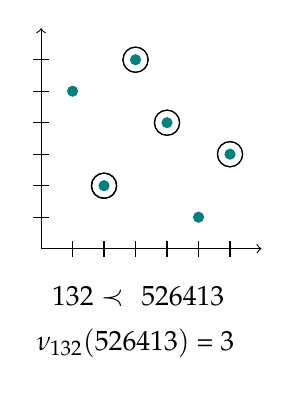
\begin{tikzpicture}[scale = .4,
                        dot/.style={circle, fill=teal, inner sep=.5mm}]
      \draw[->] (0,0) -- (7,0);
      \draw[->] (0,0) -- (0,7);
      \foreach \y [count = \x] in {5,2,6,4,1,3}{
        \node[dot] at (\x,\y) {};
        \draw (\x, -.25) -- (\x,.25);
        \draw (-.25, \x) -- (.25, \x);
      }

      \uncover<4>{
        \draw (2,2) circle (4mm);
        \draw (3,6) circle (4mm);
        \draw (6,3) circle (4mm);
      }

      \uncover<5>{
        \draw (2,2) circle (4mm);
        \draw (3,6) circle (4mm);
        \draw (4,4) circle (4mm);
      }

      \uncover<6>{
        \draw (2,2) circle (4mm);
        \draw (4,4) circle (4mm);
        \draw (6,3) circle (4mm);
      }

      \node at (4.5,-1.5) {$ 526413 $};
      \node at (1.5, -1.5) {$ 132 \prec $};

      \uncover<3->{
        \node at (3, -3) {$\nu_{132}(526413)$ = 3};
      }
    \end{tikzpicture}
    \end{center}
    }
  \end{frame}



  \begin{frame}{Random Data}
    \begin{center}
      \begin{tikzpicture}[scale=4, only marks]
      \draw (-0.05,-0.05) -- (1.05,-0.05) -- (1.05,1.05) -- (-0.05,1.05) -- cycle;
      \draw plot[mark=*, mark size = .1mm] file {organizeddata.txt};
      \end{tikzpicture}
    \end{center}

    \vspace{-1pc}

    
    \pause
    $$
    \rowcolors{1}{teal!0}{teal!10}
    \begin{array}{cc|c}
      \num_{12} &\num_{21} & \text{Avg}\\
      2803 & 2147 & 2475
    \end{array}
    $$
    \pause
    $$
    \rowcolors{1}{teal!0}{teal!10}
    \begin{array}{cccccc|c}
      \num_{123} &\num_{132} &\num_{213} &\num_{231} 
        &\num_{312} &\num_{321} & \text{Avg}\\
      35357 & 30063 & 31414 & 22321 & 23348 & 19197 & 26950
    \end{array}
    $$

  \end{frame}


  \begin{frame}{Patterns as Random Variables}
    \begin{block}{Theorem (B\'ona 2007)}
      For a (uniformly) randomly selected permutation of length $n$, 
      the random variables $\num_{\sg}$ are asymptotically normal as $n$
      approaches infinity.
    \end{block}

    \begin{block}{Theorem (Janson, Nakamura, Zeilberger 2013)}
      For a randomly selected permutation of length $n$ and two patterns $\sg$
      and $\rho$, the random variables $\num_{\sg}$ and $\num_{\rho}$ are
      asymptotically jointly normally distributed as $n \rightarrow \infty$. 
    \end{block}
  \end{frame}



  \begin{frame}{Motivation}
    \begin{block}{Fact}
      In $\S_n$, the number of occurrences of a specific pattern depends only on
      the length of the pattern. That is, for a pattern $\sg \in \S_k$, we have 
      $$ \num_{\sg} (\S_n) = \frac{n!}{k!} \binom{n}{k}.$$
    \end{block}

    \pause
    \begin{block}{Question}
    How does this change when we replace $\S_n$ with a 
    proper permutation class?
    \end{block}
    \pause

    \begin{figure}
    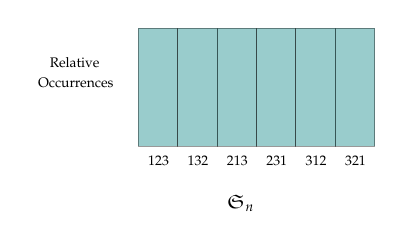
\begin{tikzpicture}
    [scale = .5]
    \foreach \x in {0,1,2,3,4,5}{
      \draw[color = black, fill = teal, opacity = .4] (\x,0) rectangle (\x+1, 3);
    }
    \draw (0, 0) node[anchor=north west] {\tiny $123$};
    \draw (1, 0) node[anchor=north west] {\tiny $132$};
    \draw (2, 0) node[anchor=north west] {\tiny $213$};
    \draw (3, 0) node[anchor=north west] {\tiny $231$};
    \draw (4, 0) node[anchor=north west] {\tiny $312$};
    \draw (5, 0) node[anchor=north west] {\tiny $321$};
    \draw (2,-1) node[anchor=north west] {\scriptsize $\S_n$};
    \draw (-2.5, 2.5) node[anchor=north west] {\tiny Relative};
    \draw (-2.8, 2) node[anchor=north west] {\tiny Occurrences};
    \end{tikzpicture} \hspace{2pc} \pause
    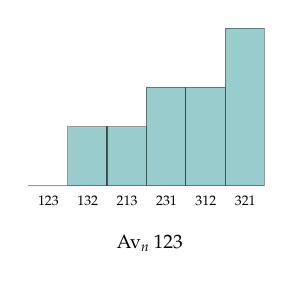
\begin{tikzpicture}
    [scale = .5]
    \foreach \x/\y in {0/0, 1/1.5, 2/1.5, 3/2.5, 4/2.5, 5/4}{
      \draw[color = black, fill = teal, opacity = .4] (\x,0) rectangle (\x+1,\y );
    }
    \draw (0, 0) node[anchor=north west] {\tiny $123$};
    \draw (1, 0) node[anchor=north west] {\tiny $132$};
    \draw (2, 0) node[anchor=north west] {\tiny $213$};
    \draw (3, 0) node[anchor=north west] {\tiny $231$};
    \draw (4, 0) node[anchor=north west] {\tiny $312$};
    \draw (5, 0) node[anchor=north west] {\tiny $321$};
    \draw (2,-1) node[anchor=north west] {\scriptsize $\Av_n 123$};
    \end{tikzpicture}
    \end{figure}
  \end{frame}

  \begin{frame}{Previous Results}

    \begin{block}{Theorem (B\'ona)}
      In $\Av_n 132$, the pattern $123$ is the least common, $321$ is the most
      common, and $\num_{213} = \num_{231} = \num_{312}$. \\
    \end{block}
      
  \end{frame}


  \begin{frame}{Data}
    \pause
    \vspace{-1pc}
    $$ \Av 132 $$
    \rowcolors{2}{teal!0}{teal!10}
    $$\begin{array}{ccccccc}
        \text{length} & 123 & 132 & 213 & 231
        & 312 & 321 \\
       3  & 1     &    0  &    1 &    1 &    1 &    1  \\
       4  & 10    &    0  &   11 &   11 &   11 &   13  \\
       5  & 68    &    0  &   81 &   81 &   81 &  109  \\
       6  & 392   &    0  &  500 &  500 &  500 &  748  \\ 
       7  & 2063  &    0  & 2794 & 2794 & 2794 & 4570   
     \end{array}
    $$
    \pause
    $$\Av 123 $$
    \rowcolors{2}{teal!0}{teal!10}
    $$\begin{array}{ccccccc}
        \text{length} & 123 & 132 & 213 & 231
        & 312 & 321 \\
        3  & 0     &    1  &    1 &    1 &    1 &    1  \\
        \pause
        4  & 0     &    9  &    9 &   11 &   11 &   16  \\
        \pause
        5  & 0     &    57 &   57 &   81 &   81 &  144  \\
        6  & 0     &   312 &  312 &  500 &  500 & 1016  \\ 
        7  & 0     &  1578 & 1578 & 2794 & 2794 & 6271   
      \end{array}
    $$
  \end{frame}

  \begin{frame} \frametitle{Patterns Within $\Av(123)$} \pause

    \begin{block}{Theorem}
      The total nuber of $231$ (and $312$) patterns is identical within the
      sets $\Av_n(123)$ and $\Av_n(132)$. 
      \pause

      Further, within $\Av_n(123)$, 

      $$ \begin{aligned}
         \num_{132} =  \num_{213} &\sim \sqrt{\frac{n}{\pi}} 4^n, \\
         \num_{231} = \num_{312}  &\sim \frac{n}{2} 4^n,  \\
         \text{and} \quad \num_{321} &\sim \frac{8}{3} \sqrt{\frac{n^3}{\pi}} 4^n.
      \end{aligned} $$
    \end{block}


  \end{frame}

  \begin{frame} \frametitle{Sketch of Proof: Patterns in Av(123)} \pause
    \begin{center}
    \begin{tikzpicture}[scale=.6]
      \node at (-2,0) {};
      \node at (13,0) {};
      \node at (5,-4) {};
      \node at (5,4) {};
      \only<2>{ 
      \node (132) at (0,0) {$\num_{132}$};
      \node (213) at (2,0) {$\num_{213}$};
      \node (231) at (4,0) {$\num_{231}$};
      \node (312) at (6,0) {$\num_{312}$};
      \node (321) at (8,0) {$\num_{321}$};
      }
      \only<3>{ 
      \node (132) at (0,0) {$\num_{132}$};
      \node at (1,0) {$+$};
      \node (213) at (2,0) {$\num_{213}$};
      \node at (3,0) {$+$};
      \node (231) at (4,0) {$\num_{231}$};
      \node at (5,0) {$+$};
      \node (312) at (6,0) {$\num_{312}$};
      \node at (7,0) {$+$};
      \node (321) at (8,0) {$\num_{321}$};
      \node at (9,0) {$=$};
      \node (321) at (10.5,0) {$\displaystyle \binom{n}{3} c_n $};
      \node at (5,-2) 
      {\small{(Both sides count the number of length three patterns)}};
      }
      \only<4>{ 
      \node (132) at (0,0) {$2\num_{132}$};
      \node at (1,0) {$+$};
      \node (213) at (2,0) {$2\num_{213}$};
      \node at (3,0) {$+$};
      \node (231) at (4,0) {$\num_{231}$};
      \node at (5,0) {$+$};
      \node (312) at (6,0) {$\num_{312}$};
      \node at (9,0) {$=$};
      \node (321) at (11,0) {$\displaystyle (n-2) \num_{12} $};
      \node at (5,-2) 
      {\small{(Count triples containing a $12$ pattern \ldots)}};
      }
      \only<5>{
      \node (132) at (0,0) {$\num_{132}$};
      \node (213) at (2,0) {$\num_{213}$};
      \node (231) at (4,0) {$\num_{231}$};
      \node (312) at (6,0) {$\num_{312}$};
      \node (321) at (8,0) {$\num_{321}$};
      \draw[rounded corners] 
        (-1, -1.5) -- (-1,1.5) -- (9,1.5) -- (9,-1.5) -- cycle;
      \draw[rounded corners] 
        (-.75, -1) -- (-.75,1) -- (6.75,1) -- (6.75,-1) -- cycle;
      }
      \only<6>{ 
      \node (132) at (0,0) {$\num_{132}$};
      \node at (1,0) {$=$};
      \node (213) at (2,0) {$\num_{213}$};
      \node (231) at (4,0) {$\num_{231}$};
      \node at (5,0) {$=$};
      \node (312) at (6,0) {$\num_{312}$};
      \node (321) at (8,0) {$\num_{321}$};
      \draw[rounded corners] 
        (-1, -1.5) -- (-1,1.5) -- (9,1.5) -- (9,-1.5) -- cycle;
      \draw[rounded corners] 
        (-.75, -1) -- (-.75,1) -- (6.75,1) -- (6.75,-1) -- cycle;
      \node at (5,-2.5) 
      {\small{(Since $\Av(123)$ is closed under inversion)}};
      }
      \only<7-8>{ 
      \node (132) at (0,0) {$\num_{213}$};
      \node (231) at (4,0) {$\num_{231}$};
      \node (321) at (8,0) {$\num_{321}$};
      \draw[rounded corners] 
        (-1, -1.5) -- (-1,1.5) -- (9,1.5) -- (9,-1.5) -- cycle;
      \draw[rounded corners] 
        (-.75, -1) -- (-.75,1) -- (6.75,1) -- (6.75,-1) -- cycle;
      \only<8>{
      \draw[rounded corners] 
        (-.65, -.75) -- (-.65,.75) -- (.65,.75) -- (.65,-.75) -- cycle;
      }
      }

    \end{tikzpicture}
    \end{center}
  \end{frame}


    

    % \begin{frame}{Sketch of Proof: Indecomposable Permutations}
    % \pause
    %   
    %   \begin{block}{Definition}
    %     We say that a permutation $p = p_1 p_2 \ldots p_n$ is
    %     \emph{decomposable} if there exists an integer $k$ so that each
    %     of the entries $p_1, \ldots p_k$ is greater than each of the
    %     entries $p_{k+1}, \ldots p_n$. Otherwise, we say that $p$ is
    %     \emph{indecomposable}
    %   \end{block}
    % 
    %   \pause
    % 
    %   \begin{block}{Example}
    %     The permutation $3 5 6 4 1 2$ is decomposable, as the entries
    %     $3564$ are larger than the entries $12$
    %   \end{block}
    % 
    %   \pause
    % 
    %   \begin{block}{Definition}
    %     Denote by $\Avns$ the set of indecomposable $n$-permutations which
    %     avoid $123$.
    %   \end{block}
    % 
    % \end{frame}
    % 
    % 
    % \begin{frame}{Sketch of Proof: Indecomposable Permutations}
    % 
    %   \begin{block}{Fact}
    %     $|\Avns| = c_{n-1}$.
    %   \end{block}
    %   \pause
    % 
    %   \begin{proof}
    %     \vspace{.5pc}
    % 
    %     \begin{tikzpicture}[scale = .45]
    %       
    %       \draw[thick] (0,8) -- (0,0) -- (8,0) -- (8,8) -- (0,8);
    %       \node at (4,4) {$\Avn$};
    %       \node at (9,4) {$ = $};
    % 
    %       \draw (10,8) -- (10,6) -- (12,6) -- (12,8) -- (10,8);
    %       \node at (11,7) {\tiny $ \Avns$};
    % 
    %       \draw (12,6) -- (12,4) -- (14,4) -- (14,6) -- (12,6);
    %       \node at (13,5) {\tiny $ \Avns$};
    %       
    %       \node at (15,3) {$\ddots$};
    % 
    %       \draw (16,2) -- (16,0) -- (18,0) -- (18,2) -- (16,2);
    %       \node at (17,1) {\tiny $ \Avns$};
    %     \end{tikzpicture}
    % 
    %     \pause
    %     $$ C(x) = 1 + C^*(x) + C^*(x)^2 + \ldots = \frac{1}{1 - C^*(x)}$$
    % 
    %     \vspace{-.5pc}
    %     \pause
    %     $$ C^*(x) = \frac{C(x) - 1}{C(x)} = \frac{(xC(x)^2 + 1) - 1}{C(x)}=  xC(x).$$
    % 
    % 
    %   \end{proof}
    % 
    % \end{frame}
    % 
    % 
    % \begin{frame}{Sketch of Proof: Indecomposable Permutations}
    % 
    %   \begin{block}{Fact}
    %     $|\Avns| = c_{n-1}$.
    %   \end{block}
    % 
    %   \begin{proof}[Alternate Proof]
    %     \vspace{.5pc}
    % 
    %     \begin{tikzpicture}[scale = .45]
    %       
    %       \draw[thick] (0,8) -- (0,0) -- (8,0) -- (8,8) -- (0,8);
    %       \node at (4,4) {$\Avn$};
    %       \node at (9,4) {$ = $};
    % 
    %       \draw (10,8) -- (10,6) -- (12,6) -- (12,8) -- (10,8);
    %       \node at (11,7) {\tiny $ \Avns$};
    % 
    %       \draw (12,6) -- (12,0) -- (18,0) -- (18,6) -- (12,6);
    %       \node at (15,3) {$ \Avn$};
    %     \end{tikzpicture}
    % 
    %     $$ C(x) = C^*(x) C(x) + 1$$
    %     
    %     \vspace{-.5pc}
    %     $$ C^*(x) = \frac{C(x) - 1}{C(x)} = \frac{(xC(x)^2 + 1) - 1}{C(x)}=  xC(x).$$
    % 
    % 
    %   \end{proof}
    % 
    % \end{frame}



  \begin{frame}{Sketch of Proof: Counting $213$ Patterns}

    \only<-12>{
      Let $p = 4 \ 3 \ 7 \ 6 \ 1 \ 5 \ 2 $, and count $213$ patterns. \\
      \hfill 
    }
    \only<13->{ Let $h_{n,k}$ denote the total number of peaks at height
    $k$ in all Dyck paths of semilength $n$. 
    Let $H(x,u) = \sum_{n,k \geq 0} h_{n,k} x^n u^k$. \\
    \vspace{-.4pc} }

    \begin{figure}[center]
    
    % lots of pictures... not the prettiest code
      \only<1>{
        \begin{tikzpicture}[scale = .7, auto = center]
          \draw[thick, color =  white] (0,8) -- (0,0) -- (8,0);
        \end{tikzpicture}
        }

      \only<2>{
        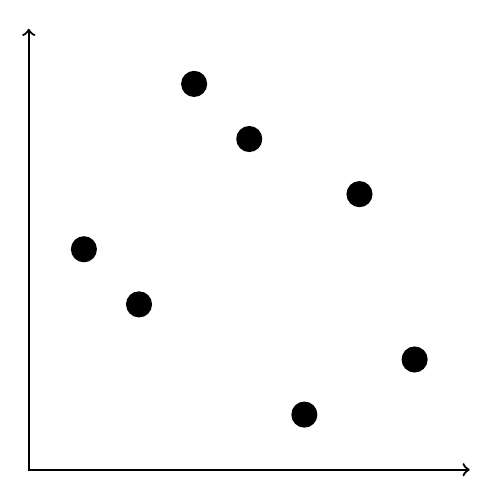
\begin{tikzpicture}[scale = .7, auto = center]
          \draw[thick, <->] (0,8) -- (0,0) -- (8,0);
          \node[circle, fill=black] at (1,4) {};
          \node[circle, fill=black] at (2,3) {};
          \node[circle, fill=black] at (3,7) {};
          \node[circle, fill=black] at (4,6) {};
          \node[circle, fill=black] at (5,1) {};
          \node[circle, fill=black] at (6,5) {};
          \node[circle, fill=black] at (7,2) {};
        \end{tikzpicture}
      }

      \only<3>{ 
        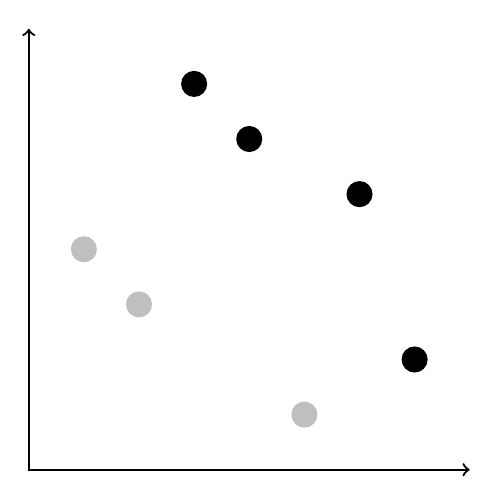
\begin{tikzpicture}[scale = .7, auto = center]
          \draw[thick, <->] (0,8) -- (0,0) -- (8,0);
          \node[circle, fill=lightgray] at (1,4) {};
          \node[circle, fill=lightgray] at (2,3) {};
          \node[circle, fill=black] at (3,7) {};
          \node[circle, fill=black] at (4,6) {};
          \node[circle, fill=lightgray] at (5,1) {};
          \node[circle, fill=black] at (6,5) {};
          \node[circle, fill=black] at (7,2) {};
        \end{tikzpicture}
      }

      \only<4>{ 
        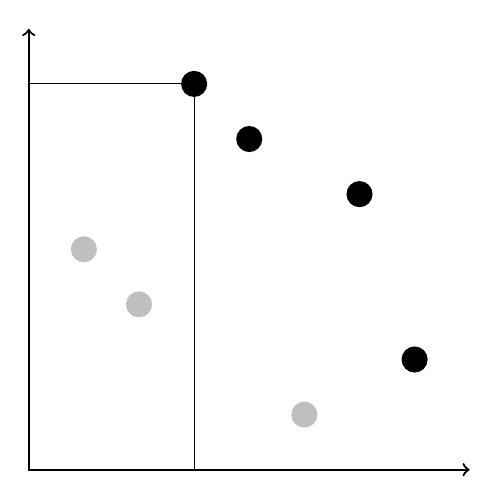
\begin{tikzpicture}[scale = .7, auto = center]
          \draw[thick, <->] (0,8) -- (0,0) -- (8,0);
          \node[circle, fill=lightgray] at (1,4) {};
          \node[circle, fill=lightgray] at (2,3) {};
          \node[circle, fill=black] at (3,7) {};
          \node[circle, fill=black] at (4,6) {};
          \node[circle, fill=lightgray] at (5,1) {};
          \node[circle, fill=black] at (6,5) {};
          \node[circle, fill=black] at (7,2) {};
          \draw (0,7) -- (3,7) -- (3,0);
        \end{tikzpicture}
      }

      \only<5>{ 
        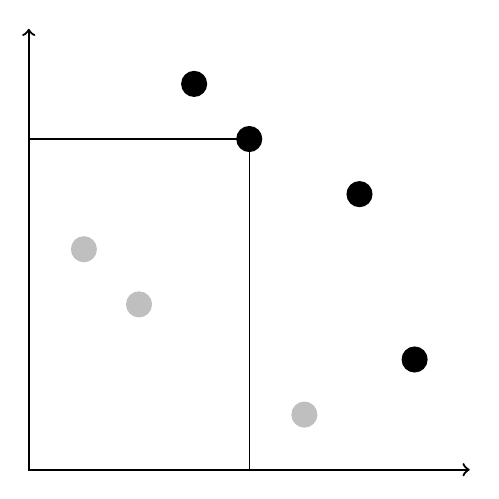
\begin{tikzpicture}[scale = .7, auto = center]
          \draw[thick, <->] (0,8) -- (0,0) -- (8,0);
          \node[circle, fill=lightgray] at (1,4) {};
          \node[circle, fill=lightgray] at (2,3) {};
          \node[circle, fill=black] at (3,7) {};
          \node[circle, fill=black] at (4,6) {};
          \node[circle, fill=lightgray] at (5,1) {};
          \node[circle, fill=black] at (6,5) {};
          \node[circle, fill=black] at (7,2) {};
          \draw (0,6) -- (4,6) -- (4,0);
        \end{tikzpicture}
      }

      \only<6>{ 
        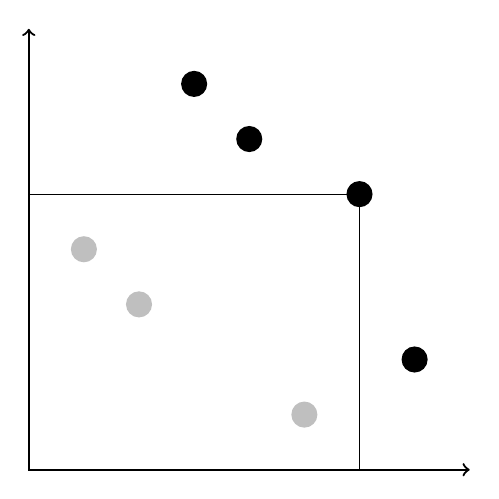
\begin{tikzpicture}[scale = .7, auto = center]
          \draw[thick, <->] (0,8) -- (0,0) -- (8,0);
          \node[circle, fill=lightgray] at (1,4) {};
          \node[circle, fill=lightgray] at (2,3) {};
          \node[circle, fill=black] at (3,7) {};
          \node[circle, fill=black] at (4,6) {};
          \node[circle, fill=lightgray] at (5,1) {};
          \node[circle, fill=black] at (6,5) {};
          \node[circle, fill=black] at (7,2) {};
          \draw (0,5) -- (6,5) -- (6,0);
        \end{tikzpicture}
      }

      \only<7>{ 
        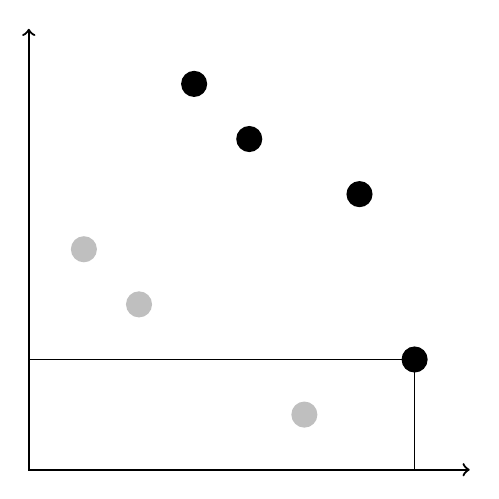
\begin{tikzpicture}[scale = .7, auto = center]
          \draw[thick, <->] (0,8) -- (0,0) -- (8,0);
          \node[circle, fill=lightgray] at (1,4) {};
          \node[circle, fill=lightgray] at (2,3) {};
          \node[circle, fill=black] at (3,7) {};
          \node[circle, fill=black] at (4,6) {};
          \node[circle, fill=lightgray] at (5,1) {};
          \node[circle, fill=black] at (6,5) {};
          \node[circle, fill=black] at (7,2) {};
          \draw (0,2) -- (7,2) -- (7,0);
        \end{tikzpicture}
      }

      \only<8>{ 
        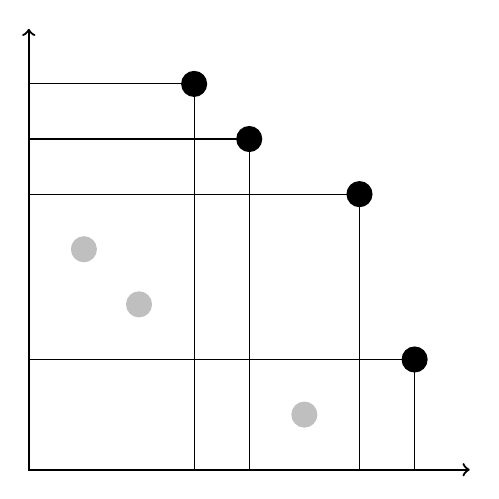
\begin{tikzpicture}[scale = .7, auto = center]
          \draw[thick, <->] (0,8) -- (0,0) -- (8,0);
          \node[circle, fill=lightgray] at (1,4) {};
          \node[circle, fill=lightgray] at (2,3) {};
          \node[circle, fill=black] at (3,7) {};
          \node[circle, fill=black] at (4,6) {};
          \node[circle, fill=lightgray] at (5,1) {};
          \node[circle, fill=black] at (6,5) {};
          \node[circle, fill=black] at (7,2) {};
          \draw (0,7) -- (3,7) -- (3,0);
          \draw (0,6) -- (4,6) -- (4,0);
          \draw (0,5) -- (6,5) -- (6,0);
          \draw (0,2) -- (7,2) -- (7,0);
        \end{tikzpicture}
      }

      \only<9>{ 
        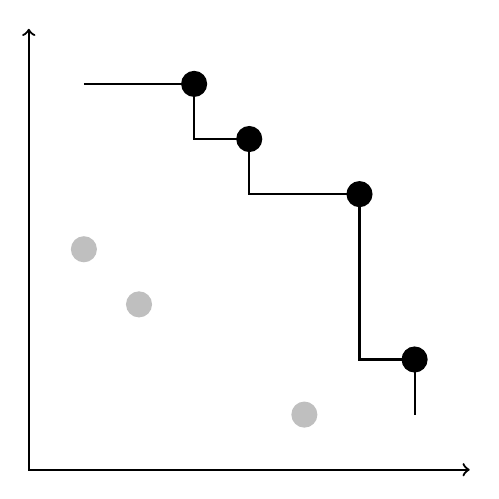
\begin{tikzpicture}[scale = .7, auto = center]
          \draw[thick, <->] (0,8) -- (0,0) -- (8,0);
          \node[circle, fill=lightgray] at (1,4) {};
          \node[circle, fill=lightgray] at (2,3) {};
          \node[circle, fill=black] at (3,7) {};
          \node[circle, fill=black] at (4,6) {};
          \node[circle, fill=lightgray] at (5,1) {};
          \node[circle, fill=black] at (6,5) {};
          \node[circle, fill=black] at (7,2) {};
          \draw[thick] (1,7) -- (3,7) -- (3,6) -- (4,6) --
                       (4,5) -- (6,5) -- (6,2) -- (7,2) --
                       (7,1);
        \end{tikzpicture}
      }

      \only<10>{ 
        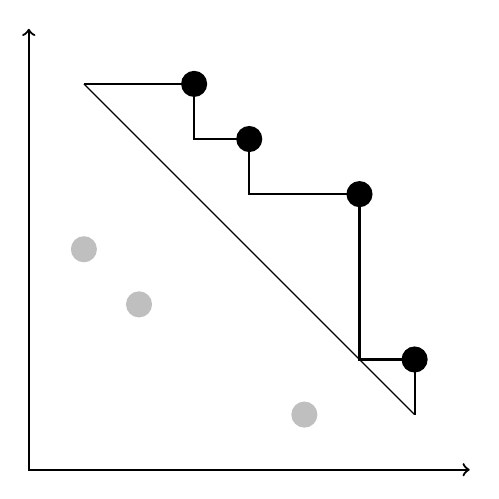
\begin{tikzpicture}[scale = .7, auto = center]
          \draw[thick, <->] (0,8) -- (0,0) -- (8,0);
          \node[circle, fill=lightgray] at (1,4) {};
          \node[circle, fill=lightgray] at (2,3) {};
          \node[circle, fill=black] at (3,7) {};
          \node[circle, fill=black] at (4,6) {};
          \node[circle, fill=lightgray] at (5,1) {};
          \node[circle, fill=black] at (6,5) {};
          \node[circle, fill=black] at (7,2) {};
          \draw[thick] (1,7) -- (3,7) -- (3,6) -- (4,6) --
                       (4,5) -- (6,5) -- (6,2) -- (7,2) --
                       (7,1);
          \draw (1,7) -- (7,1);
        \end{tikzpicture}
      }

      \only<11>{
        \begin{tikzpicture}[scale = .7, auto = center]
          \draw[thick, color =  white] (0,8) -- (0,0) -- (8,0);
          \draw[thick] (0,2) -- (2,4) -- (3,3) -- (4,4) --
                       (5,3) -- (7,5) -- (10,2) -- (11,3) --
                       (12,2);
          \draw (0,2) -- (12,2);
        \end{tikzpicture}
      }

      \only<12,13>{
        \begin{tikzpicture}[scale = .7, auto = center]
          \draw[thick, color =  white] (0,8) -- (0,0) -- (8,0);
          \draw[thick] (0,2) -- (2,4) -- (3,3) -- (4,4) --
                       (5,3) -- (7,5) -- (10,2) -- (11,3) --
                       (12,2);
          \draw (0,2) -- (12,2);
          
          \node at (2,5) {2};
          \node at (4,5) {2};
          \node at (7,6) {3};
          \node at (11,4) {1};
        \end{tikzpicture}
      }

      \only<14>{
        \begin{tikzpicture}[scale = .7, auto = center]
          \draw[thick, color =  white] (0,8) -- (0,0) -- (8,0);
          \draw[thick] (0,2) -- (2,4) -- (3,3) -- (4,4) --
                       (5,3) -- (7,5) -- (10,2) -- (11,3) --
                       (12,2);
          \draw (0,2) -- (12,2);
          \draw (1,3) -- (9,3);
          \draw (10,1) -- (10,5);
        \end{tikzpicture}
      }

      \only<15>{
        \vspace{.1pc}

        \begin{tikzpicture}[scale = .7, auto = center]
          \draw[thick, color =  white] (0,8) -- (0,0) -- (8,0);
          \draw[thick] (0,2) -- (2,4) -- (3,3) -- (4,4) --
                       (5,3) -- (7,5) -- (10,2) -- (11,3) --
                       (12,2);
          \draw (0,2) -- (12,2);
          \draw (1,3) -- (9,3);
          \draw (10,1) -- (10,5);

          \node at (5,5) {$uH(x,u)$};
          \node at (11,5) {$H(x,u)$};
        \end{tikzpicture}
      }

    \end{figure}


      $$ \only<4-13>{\num_{213}(p)}  \uncover<4-13>{ = \binom{2}{2}}
      \only<5-13>{ + \binom{2}{2}} \only<6-13>{ + \binom{3}{2}}
      \only<7-13>{ + \binom{1}{2}} \only<8-13>{ = 5  }
      \only<14->{H(x,u) = } 
      \only<15->{ux (H(x,u) + 1) C(x) + xC(x) H(x,u)}  
      $$ 

  \end{frame}


  \begin{frame}{Sketch of Proof: Counting $213$ Patterns}

    Let $h_{n,k}$ denote the total number of peaks at height
    $k$ in all Dyck paths of semilength $n$. 
    Let $H(x,u) = \sum_{n,k \geq 0} h_{n,k} x^n u^k$. 
    
    \vspace{2pc}

    $$ \begin{aligned}
    H(x,u) &= \frac{uxC(x)}{1-uxC(x)-xC(x)}. \\
    \pause
    \sum_{n \geq 0} \num_{213}(\Av_n^*(123))x^n  
      &= \sum_{n \geq 0} \binom{k}{2} h_{n-1,k} x^n \\
    \pause
    \sum_{n \geq 0} \num_{213}(\Av_n^*(123))x^n  
      &= \frac{\left. x \partial_u ^2 H(x)\right|_{u=1}}{2} \\
           \pause
           &= \frac{x^3C(x)}{(1-4x)^{3/2}} \\ 
           \pause
           &= x^3 + 7x^4 + 38x^5 + 187^6 + \ldots
        \end{aligned} $$
      \pause
      \begin{flushright} $ \qed $ \end{flushright}

  \end{frame}


  \begin{frame}{Results}
    \pause
      $$ \num_{231}(\Av_n 123) = \num_{231}(\Av_n 132)$$
  \end{frame}

  \begin{frame}{Results}

    $$ \nu_{213} = \frac{n+2}{4} \binom{2n}{n} - 3 \cdot 2^{2n-3} $$\\[.5pc]
    $$ \nu_{231} = (2n-1) \binom{2n-3}{n-2} - (2n+1)\binom{2n-1}{n-1} + 
       (n+4) \cdot 2^{2n-3}$$\\[.5pc]
    $$ \begin{aligned} \nu_{321} 
        &= \frac{1}{6} \binom{2n+5}{n+1} \binom{n+4}{2} 
        - \frac{5}{3} \binom{2n+3}{n} \binom{n+3}{2} \\
        &+ \frac{17}{3} \binom{2n+1}{n-1} \binom{n+2}{2} 
        - 6\binom{2n-1}{n-2} \binom{n+1}{2} - (n+1) \cdot 4^{n-1}.
      \end{aligned}
    $$

  \end{frame}




  \begin{frame}{Further Directions/Applications}
    \pause
    \begin{block}{Question}
      Are there any other `surprising' symmetries across or within permutation
      classes?
    \end{block}

    \pause

    \begin{block}{Note}
      The increasing and decreasing patterns are not always the opposite extremes of the
      class: $\num_{123} (\Av 2413) = \num_{321} (\Av 2413) $ 
    \end{block}
    \pause

    \vspace{1pc}

    \begin{center}
    \begin{tikzpicture}
    [scale = .5]
    \foreach \x/\y in {0/3,1/2,2/2,3/2,4/2,5/3}{
      \draw[color = black, fill = teal, opacity = .4] (\x,0) rectangle (\x+1,\y);
    }
    \draw (0, 0) node[anchor=north west] {\tiny $123$};
    \draw (1, 0) node[anchor=north west] {\tiny $132$};
    \draw (2, 0) node[anchor=north west] {\tiny $213$};
    \draw (3, 0) node[anchor=north west] {\tiny $231$};
    \draw (4, 0) node[anchor=north west] {\tiny $312$};
    \draw (5, 0) node[anchor=north west] {\tiny $321$};
    \draw (2,-1) node[anchor=north west] {\scriptsize $\Av 2413$};
    \draw (-2.5, 2.5) node[anchor=north west] {\tiny Relative};
    \draw (-2.8, 2) node[anchor=north west] {\tiny Occurrences};
    \end{tikzpicture} 
    \end{center}

    \pause
    \begin{block}{Question}
      What about multiset permutations?
    \end{block}

  \end{frame}



  \section{Genome Rearrangement}
  \begin{frame}
    \centering
    \Large \color{teal}{Genome Rearrangement}
  \end{frame}



  \begin{frame}{Evolutionary Distance}
    \begin{center}
    \begin{tikzpicture}[scale=.9]
      \uncover<2->{
      \node (duck) at (0,0) {\includegraphics[width=6pc]{images/duck.png}};
      \node (duckmom) at (.5,2) {};
      \node (beaver) at (8,0) {\includegraphics[width=6pc]{images/beaver.png}};
      \node (beavermom) at (7.5,2) {};
      }

      \uncover<3->{
      % \node (plat) at (4, 6) 
      %   {\only<2-3>{\Large ?}
      %    \only<4->{\includegraphics[width=6pc]{images/platypus.png}}
      %   };
      \only<3-4>{\node (plat) at (4, 6) {\Large ?};}
      \uncover<5->{\node (plat) at (4,6)
        {\includegraphics[width=6pc]{images/platypus.png}};}

      \draw[thin] (plat) -- (3,4);
      \draw[thin] (plat) -- (3.7,4);
      \draw[thin] (plat) -- (4.3,4);
      \draw[thin] (plat) -- (5,4);
      \draw[thin] (3,4) -- (2.7, 3.5);
      \draw[thin] (3,4) -- (3, 3.5);
      \draw[thin] (3,4) -- (3.3, 3.5);

      \draw[thin] (3.7,4) -- (3.5, 3.5);
      \draw[thin] (3.7,4) -- (3.9, 3.5);

      \draw[thin] (4.3,4) -- (4.3, 3.5);

      \draw[thin] (5,4) -- (4.8, 3.5);
      \draw[thin] (5,4) -- (5.2, 3.5);

      \uncover<4->{
        \draw[ultra thick] (duck) -- (duckmom);
        \draw[ultra thick] (beaver) -- (beavermom);
        \draw[ultra thick] (plat) -- (3,4) -- (3,3.5);
        \draw[ultra thick] (plat) -- (5,4) -- (5.2,3.5);
        \draw[ultra thick, dotted] (duckmom) -- (3,3.5);
        \draw[ultra thick, dotted] (beavermom) -- (5.2,3.5);
      }



      \only<3>{\draw[dotted] (2, 3) -- (6,3);}
      \only<3>{\draw[dotted] (1.7, 2.75) -- (6.3,2.75);}
      \only<3>{\draw[dotted] (1.5, 2.5) -- (6.5,2.5);}
      \draw (duckmom) -- (duck);
      \draw (beavermom) -- (beaver);



      }
    \end{tikzpicture}
    \end{center}
  \end{frame}

  \begin{frame}{Genome Rearrangement} 
    \begin{center}
    \begin{tikzpicture}[scale=.5]
      \draw[white] (0,-5) -- (15,-5) -- (15,4) -- (0, 4) -- cycle;

      \only<1>{
        \draw[fill = teal!25, rounded corners]
          (0,1) -- (15,1) -- (15, 0) -- (0,0) -- cycle;
        \node at (8.1,-1) {$CCGTGCTACACTGCGATCCGACT \dots$};
      }

      \only<2>{
        \draw[fill = teal!25, rounded corners]
          (0,1) -- (3,1) -- (3, 0) -- (0,0) -- cycle;
        \draw[fill = white, rounded corners]
          (3,1) -- (6,1) -- (6, 0) -- (3,0) -- cycle;
        \draw[fill = teal!25, rounded corners]
          (6,1) -- (15,1) -- (15, 0) -- (6,0) -- cycle;
        \node at (8.1,-1) {$CCG\boxed{TGCTA}CACTGCGATCCGACT \dots$};
      }

      \only<3>{
        \draw[fill = teal!25, rounded corners]
          (0,1) -- (3,1) -- (3, 0) -- (0,0) -- cycle;
        \draw[fill = white, rounded corners]
          (3,1) -- (6,1) -- (6, 0) -- (3,0) -- cycle;
        \draw[fill = teal!25, rounded corners]
          (6,1) -- (15,1) -- (15, 0) -- (6,0) -- cycle;
        \node at (8.1,-1) {$CCG\boxed{TGCTA}CACTGCGATCCGACT \dots$};

        \draw[dotted] (11,-.5) -- (11,1.5);
        \draw[->] (4.5,1.5) .. controls (4.5, 3) and (11,3) .. (11,1.5);
      }
      \only<4>{
        \draw[fill = teal!25, rounded corners]
          (0,1) -- (4.5,1) -- (4.5, 0) -- (0,0) -- cycle;
        \draw[fill = teal!25, rounded corners]
          (4.5,1) -- (8,1) -- (8, 0) -- (4.5,0) -- cycle;
        \draw[fill = white, rounded corners]
          (8,1) -- (11,1) -- (11, 0) -- (8,0) -- cycle;
        \draw[fill = teal!25, rounded corners]
          (11,1) -- (15,1) -- (15, 0) -- (11,0) -- cycle;
        \node at (8.1,-1) {$CCGCACTGCGATC\boxed{TGCTA}CGACT \dots$};

        \draw[->] (4.5,1.5) .. controls (4.5, 3) and (9.5,3) .. (9.5,1.5);
      }
    \end{tikzpicture}
    \end{center}
  \end{frame}


  \begin{frame}{Block Transformations}
    % \setbeamercovered{transparent}
    \begin{center}
    \begin{tikzpicture}[scale=.3]
      \draw[fill = teal!25, rounded corners]
        (0,1) -- (2,1) -- (2, 0) -- (0,0) -- cycle;
      \draw[fill = white, rounded corners]
        (2,1) -- (4,1) -- (4, 0) -- (2,0) -- cycle;
      \draw[fill = teal!25, rounded corners]
        (4,1) -- (8,1) -- (8, 0) -- (4,0) -- cycle;
      \draw[dotted] (6,-.5) -- (6,1.5);
      \draw[->] (3,1.5) .. controls (3, 3) and (6,3) .. (6,1.5);
      \node at (4,-1) {\small Block Transposition};
    \end{tikzpicture}
    \uncover<2>{
    \hspace{1pc}
    \begin{tikzpicture}[scale=.3]
      \draw[fill = teal!25, rounded corners]
        (0,1) -- (2,1) -- (2, 0) -- (0,0) -- cycle;
      \draw[fill = white, rounded corners]
        (2,1) -- (4,1) -- (4, 0) -- (2,0) -- cycle;
      \draw[fill = teal!25, rounded corners]
        (4,1) -- (8,1) -- (8, 0) -- (4,0) -- cycle;
      \draw[->] (3,1.5) .. controls (1, 4) and (5,4) .. (3.2,1.5);
      \node at (3,4) {\scriptsize $-1$};
      \node at (4,-1) {\small Block Reversal};
    \end{tikzpicture}
    \hspace{1pc}
    \begin{tikzpicture}[scale=.3]
      \draw[fill = teal!25, rounded corners]
        (0,1) -- (2,1) -- (2, 0) -- (0,0) -- cycle;
      \draw[fill = white, rounded corners]
        (2,1) -- (4,1) -- (4, 0) -- (2,0) -- cycle;
      \draw[fill = teal!25, rounded corners]
        (4,1) -- (6,1) -- (6, 0) -- (4,0) -- cycle;
      \draw[fill = white, rounded corners]
        (6,1) -- (8,1) -- (8, 0) -- (6,0) -- cycle;
      \draw[fill = teal!25, rounded corners]
        (8,1) -- (10,1) -- (10, 0) -- (8,0) -- cycle;

      \draw[<->] (3,1.5) .. controls (3, 3) and (7,3) .. (7,1.5);
      \node at (5,-1) {\small Block Interchange};
    \end{tikzpicture}

    \vspace{1pc}

    \begin{tikzpicture}[scale=.3]
      \draw[fill = white, rounded corners]
        (0,1) -- (2,1) -- (2, 0) -- (0,0) -- cycle;
      \draw[fill = teal!25, rounded corners]
        (2,1) -- (8,1) -- (8, 0) -- (2,0) -- cycle;
      \draw[dotted] (6,-.5) -- (6,1.5);
      \draw[->] (1,1.5) .. controls (1, 3) and (6,3) .. (6,1.5);
      \node at (4,-1) {\small Prefix Transposition};
    \end{tikzpicture}
    %\hspace{1pc}
    %
    \begin{tikzpicture}[scale=.3]
      \draw[fill = white, rounded corners]
        (0,1) -- (2,1) -- (2, 0) -- (0,0) -- cycle;
      \draw[fill = teal!25, rounded corners]
        (2,1) -- (8,1) -- (8, 0) -- (2,0) -- cycle;
      \draw[->] (1,1.5) .. controls (-1, 4) and (3,4) .. (1.2,1.5);
      \node at (1,4) {\scriptsize $-1$};
      \node at (4,-1) {\small Prefix Reversal};
    \end{tikzpicture}
    \hspace{1pc}
    %
    \begin{tikzpicture}[scale=.3]
      \draw[fill = teal!25, rounded corners]
        (0,1) -- (2,1) -- (2, 0) -- (0,0) -- cycle;
      \draw[fill = white, rounded corners]
        (2,1) -- (4,1) -- (4, 0) -- (2,0) -- cycle;
      \draw[fill = teal!25, rounded corners]
        (4,1) -- (8,1) -- (8, 0) -- (4,0) -- cycle;
      \draw[dotted] (6,-.5) -- (6,1.5);
      \draw[->] (3,1.5) .. controls (3, 3) and (6,3) .. (6,1.5);
      \node at (4.5, 3.5) {\scriptsize $\{1, -1\}$}; 
      \node at (4,-1) {\small Cut and Paste};
    \end{tikzpicture}
    }
    \end{center}
  \end{frame}


  \begin{frame}{Block Transformations} 
    
    \begin{block}{Question}
      For a given block transformation, how many mutations does it take to turn
      one genome into another?
    \end{block}
    \pause

    \begin{block}{Question}
      How many block transformations does it take to turn one permutation into
      another?
    \end{block}

    \pause

    \begin{block}{Question}
      Given the increasing permutation, how many block transformations does it
      take to sort it into a given permutation?
    \end{block}
  \end{frame}

  \begin{frame}{Example: Block Transpositions}
    \only<1>{\begin{center} \includegraphics[width=20pc]{images/trans3} \end{center}}
    \only<2>{\begin{center} \includegraphics[width=20pc]{images/trans4} \end{center}}
    \only<3>{\begin{center} \includegraphics[width=20pc]{images/trans5} \end{center}}
  \end{frame}



  \begin{frame}{Block Transformations and Polynomial Classes} \pause
    
    \begin{block}{Definition}
      A \emph{polynomial class} is a class $\C$ for which $f(n) = |\C_n|$ is
      given by a polynomial for large enough $n$. 
    \end{block}

    \pause
      
    \begin{block}{Theorem}
      For a given block transformation and a positive integer $k$, the set of
      permutations which are at most $k$ transformations from the permutation $1
      2 3 \dots n$ forms a polynomial class.
    \end{block}
  \end{frame}


  \begin{frame}{Peg Figures} \pause
    \begin{block}{Definition}
      A \emph{peg figure} consists of a grid of increasing and decreasing lines
      and dots, with one non-empty cell per row and column:
    \end{block} 

    \begin{center}
      \begin{tikzpicture}[scale=.3]
        \draw (0,0) -- (12,0) -- (12,12) -- (0,12) -- cycle;
        \draw[dotted] (4,0) -- (4,12);
        \draw[dotted] (8,0) -- (8,12);
        \draw[dotted] (0,4) -- (12,4);
        \draw[dotted] (0,8) -- (12,8);
        \draw (0,8) -- (4,12);
        \draw[fill = black] (6,2) circle (2mm);
        \draw (8,8) -- (12,4);
      \end{tikzpicture}
    \end{center}
    
    \vspace{-1pc}
    \pause

    \begin{block}{Definition}
      A \emph{peg permutation} is a permutation $\overset{\sim}{\pi}$ with each
      entry decorated by either a $+$, $-$, or $\bullet$. 
    \end{block}

    \vspace{-1pc}

    \pause

    $$ \overset{\sim}{\pi} = \overset{+}{3}\ \overset{\bullet}{1}\ \overset{-}{2} $$
  \end{frame}

  \begin{frame}{Peg Classes}
    \begin{block}{Definition}
      Let $\C(\overset{\sim}{\pi})$ denote the class of permutations which can be
      drawn on the figure corresponding to $\overset{\sim}{\pi}$. 
    \end{block}

    \pause

    \begin{center}
      \begin{tikzpicture}[scale=.3]
        \draw[draw=none] (0,0) -- (12,0) -- (12,12) -- (0,12) -- cycle;
        \foreach \x/\y in {1/9, 2/10, 3/11, 6/2, 9.5/6.5, 10.5/5.5}
          \draw[fill = black] (\x,\y) circle (2mm);
      \end{tikzpicture}
      \hspace{4pc}
      \begin{tikzpicture}[scale=.3]
        \draw (0,0) -- (12,0) -- (12,12) -- (0,12) -- cycle;
        \draw[dotted] (4,0) -- (4,12);
        \draw[dotted] (8,0) -- (8,12);
        \draw[dotted] (0,4) -- (12,4);
        \draw[dotted] (0,8) -- (12,8);
        \draw (0,8) -- (4,12);
        \draw[fill = black] (6,2) circle (2mm);
        \draw (8,8) -- (12,4);
      \end{tikzpicture}
    \end{center}

    $$ 456132 \in \C(\overset{+}{3} \overset{\bullet}{1} \overset{-}{2})$$

  \end{frame}


  \begin{frame}{Polynomial Classes} 
    \begin{block}{Theorem (Vatter et. al.)}
      A permutation class is a polynomial class if and only if it can be
      expressed as the union of classes of the form $\C(\overset{\sim}{\pi})$. 
    \end{block}
    \pause
    \begin{block}{Algorithm}
      Takes peg permutations as input, and returns the
      polynomial enumerating the class.
    \end{block}

  \end{frame}

  \begin{frame}{Example: $\Av(123,231)$}
    \begin{block}{Fact}
      The class $\Av(123, 231)$ is equal to the peg class 
      $\C(\overset{-}{3} \overset{-}{1} \overset{-}{2})$. 
    \end{block}
    \begin{center} 
      \begin{tikzpicture}[scale=.3]
        \draw (0,0) -- (12,0) -- (12,12) -- (0,12) -- cycle;
        \draw[dotted] (4,0) -- (4,12);
        \draw[dotted] (8,0) -- (8,12);
        \draw[dotted] (0,4) -- (12,4);
        \draw[dotted] (0,8) -- (12,8);
        \draw (0,12) -- (4,8);
        \draw (4,4) -- (8,0);
        \draw (8,8) -- (12,4);
      \end{tikzpicture}
    \end{center}
  \end{frame}

    
  \begin{frame}{Example: $\Av(123,231)$}
    %\setbeamercovered{transparent}
    \begin{tikzpicture}[scale=.05]
        % \draw (0,0 + 5*24) -- (12,0 + 5*24) -- 
        %     (12,12 + 5*24) -- (0,12 + 5*24) -- cycle;
        % \draw[dotted] (4,0 + 5*24) -- (4,12 + 5*24);
        % \draw[dotted] (8,0 + 5*24) -- (8,12 + 5*24);
        % \draw[dotted] (0,4 + 5*24) -- (12,4 + 5*24);
        % \draw[dotted] (0,8 + 5*24) -- (12,8 + 5*24);
        % \draw (0,12 + 5*24) -- (4,8 + 5*24);
        % \draw (4,4 + 5*24) -- (8,0 + 5*24);
        % \draw (8,8 + 5*24) -- (12,4 + 5*24);



        \foreach \x/\y in {0/5}{
            \draw (\x*24 + 0,\y*24 + 0) -- 
                  (\x*24 + 12,\y*24 + 0) -- 
                  (\x*24 + 12,\y*24 + 12) -- 
                  (\x*24 + 0, \y*24 + 12) -- cycle;
            \draw[dotted] (\x*24 + 4,\y*24 + 0) -- (\x*24 + 4, \y*24 + 12);
            \draw[dotted] (\x*24 + 8,\y*24 + 0) -- (\x*24 + 8, \y*24 + 12);
            \draw[dotted] (\x*24 + 0,\y*24 + 4) -- (\x*24 + 12,\y*24 + 4);
            \draw[dotted] (\x*24 + 0,\y*24 + 8) -- (\x*24 + 12,\y*24 + 8);
        }


      % top row
        \draw (0,12 + 5*24) -- (4,8 + 5*24);
        \draw (4,4 + 5*24) -- (8,0 + 5*24);
        \draw (8,8 + 5*24) -- (12,4 + 5*24);



      \pause
      % second row
      \foreach \x/\y in {-1/4, 0/4, 1/4}{
          \draw (\x*24 + 0,\y*24 + 0) -- 
                (\x*24 + 12,\y*24 + 0) -- 
                (\x*24 + 12,\y*24 + 12) -- 
                (\x*24 + 0, \y*24 + 12) -- cycle;
          \draw[dotted] (\x*24 + 4,\y*24 + 0) -- (\x*24 + 4, \y*24 + 12);
          \draw[dotted] (\x*24 + 8,\y*24 + 0) -- (\x*24 + 8, \y*24 + 12);
          \draw[dotted] (\x*24 + 0,\y*24 + 4) -- (\x*24 + 12,\y*24 + 4);
          \draw[dotted] (\x*24 + 0,\y*24 + 8) -- (\x*24 + 12,\y*24 + 8);
      }

        %lines
        \draw (6, 5*24) -- (6 - 24, 12 + 4*24);
        \draw (6, 5*24) -- (6, 12 + 4*24);
        \draw (6, 5*24) -- (6 + 24, 12 + 4*24);

        % boxes
        \draw[fill=black] (2 - 24,10 + 4*24) circle (4mm);
        \draw (4 - 24,4 +  4*24) -- (8 - 24,0 +  4*24);
        \draw (8 - 24,8 +  4*24) -- (12 - 24,4 + 4*24);

        \draw (0,12 + 4*24) -- (4,8 +  4*24);
        \draw[fill=black] (6,2 +  4*24) circle (4mm);
        \draw (8,8 +  4*24) -- (12,4 + 4*24);

        \draw (0 + 24,12 + 4*24) -- (4 + 24,8 +  4*24);
        \draw (4 + 24,4 +  4*24) -- (8 + 24,0 +  4*24);
        \draw[fill=black] (10 + 24,6 + 4*24) circle (4mm);
      
      \pause
      % third row
        \foreach \x/\y in {-2/3, -1/3, 0/3}{
            \draw (\x*24 + 0,\y*24 + 0) -- 
                  (\x*24 + 12,\y*24 + 0) -- 
                  (\x*24 + 12,\y*24 + 12) -- 
                  (\x*24 + 0, \y*24 + 12) -- cycle;
            \draw[dotted] (\x*24 + 4,\y*24 + 0) -- (\x*24 + 4, \y*24 + 12);
            \draw[dotted] (\x*24 + 8,\y*24 + 0) -- (\x*24 + 8, \y*24 + 12);
            \draw[dotted] (\x*24 + 0,\y*24 + 4) -- (\x*24 + 12,\y*24 + 4);
            \draw[dotted] (\x*24 + 0,\y*24 + 8) -- (\x*24 + 12,\y*24 + 8);
        }
        \foreach \x/\y in {1/3, 2/3}{
            \draw (\x*24 + 0,\y*24 + 0) -- 
                  (\x*24 + 12,\y*24 + 0) -- 
                  (\x*24 + 12,\y*24 + 12) -- 
                  (\x*24 + 0, \y*24 + 12) -- cycle;
            \draw[dotted] (\x*24 + 6,\y*24 + 0) -- (\x*24 + 6, \y*24 + 12);
            \draw[dotted] (\x*24 + 0,\y*24 + 6) -- (\x*24 + 12,\y*24 + 6);
        }


        \draw (2 - 48,10 + 3*24) circle (4mm);
        \draw (6 - 48,2 +  3*24) circle (4mm);
        \draw (8 - 48,8 +  3*24) -- (12 -48,4 + 3*24);

        \draw (0-24,12 + 3*24) -- (4-24,8 +  3*24);
        \draw[fill=black] (6-24,2 +  3*24) circle (4mm);
        \draw[fill=black] (10-24,6 +  3*24) circle (4mm);


        \draw[fill=black] (2  ,10 + 3*24) circle (4mm);
        \draw (4  ,4 +  3*24) -- (8 ,0 +  3*24);
        \draw[fill=black] (10,6 + 3*24) circle (4mm);

        \draw (0 +24,12+ 3*24) -- (6+ 24, 6 + 3*24);
        \draw (6 +24,6 + 3*24) -- (12+ 24, 0 + 3*24);

        \draw (6 +48,12+ 3*24) -- (12 + 48, 6 + 3*24);
        \draw (0 +48,6 + 3*24) -- (6+ 48, 0 + 3*24);

        % lines:
        \draw (6 - 24, 4*24) -- (6 - 2*24, 12 + 3*24);
        \draw (6 - 24, 4*24) -- (6, 12 + 3*24);
        \draw (6 - 24, 4*24) -- (6 + 2*24, 12 + 3*24);
        %lines:
        \draw (6, 4*24) -- (6 - 2*24, 12 + 3*24);
        \draw (6, 4*24) -- (6 - 1*24, 12 + 3*24);
        \draw (6, 4*24) -- (6 + 1*24, 12 + 3*24);
        %lines:
        \draw (6 + 24, 4*24) -- (6 - 1*24, 12 + 3*24);
        \draw (6 + 24, 4*24) -- (6 - 0*24, 12 + 3*24);
        \draw (6 + 24, 4*24) -- (6 + 1*24, 12 + 3*24);
      
      \pause
      % fourth row

        \foreach \x/\y in {-2/2}{
            \draw (\x*24 + 0,\y*24 + 0) -- 
                  (\x*24 + 12,\y*24 + 0) -- 
                  (\x*24 + 12,\y*24 + 12) -- 
                  (\x*24 + 0, \y*24 + 12) -- cycle;
            \draw[dotted] (\x*24 + 4,\y*24 + 0) -- (\x*24 + 4, \y*24 + 12);
            \draw[dotted] (\x*24 + 8,\y*24 + 0) -- (\x*24 + 8, \y*24 + 12);
            \draw[dotted] (\x*24 + 0,\y*24 + 4) -- (\x*24 + 12,\y*24 + 4);
            \draw[dotted] (\x*24 + 0,\y*24 + 8) -- (\x*24 + 12,\y*24 + 8);
        }
        \foreach \x/\y in { -1/2, 0/2, 1/2,2/2 }{
            \draw (\x*24 + 0,\y*24 + 0) -- 
                  (\x*24 + 12,\y*24 + 0) -- 
                  (\x*24 + 12,\y*24 + 12) -- 
                  (\x*24 + 0, \y*24 + 12) -- cycle;
            \draw[dotted] (\x*24 + 6,\y*24 + 0) -- (\x*24 + 6, \y*24 + 12);
            \draw[dotted] (\x*24 + 0,\y*24 + 6) -- (\x*24 + 12,\y*24 + 6);
        }


        \draw[fill=black] (2 - 4*12,10 + 2*24) circle (4mm);
        \draw[fill=black] (6 - 4*12,2 +  2*24) circle (4mm);
        \draw[fill=black] (10- 4*12,6 +  2*24) circle (4mm); 



        \draw[fill=black] (3 - 2*12, 3 + 2*24) circle (4mm);
        \draw (6 - 2*12, 12 + 2*24) -- (12- 2*12, 6 + 2*24);

        \draw (0 + 0*12, 6+ 2*24) -- (6 + 0*12, 0 + 2*24);
        \draw[fill=black] (9 + 0*12, 9 + 2*24) circle (4mm);

        \draw[fill=black] (3 + 2*12, 9 + 2*24) circle (4mm);
        \draw (6 + 2*12, 6 + 2*24) -- (12+ 2*12, 0 + 2*24);

        \draw (0 + 4*12, 12+ 2*24) -- (6 + 4*12, 6 + 2*24);
        \draw[fill=black] (9 + 4*12, 3 + 2*24) circle (4mm);

        % lines
        \draw (6 - 2*24, 3*24) -- (6 - 2*24, 12 + 2*24);
        \draw (6 - 2*24, 3*24) -- (6 - 1*24, 12 + 2*24);
        \draw (6 - 2*24, 3*24) -- (6 + 1*24, 12 + 2*24);

        \draw (6 - 1*24, 3*24) -- (6 - 2*24, 12 + 2*24);
        \draw (6 - 1*24, 3*24) -- (6 + 2*24, 12 + 2*24);

        \draw (6 - 0*24, 3*24) -- (6 - 2*24, 12 + 2*24);
        \draw (6 - 0*24, 3*24) -- (6 + 0*24, 12 + 2*24);
        \draw (6 - 0*24, 3*24) -- (6 + 1*24, 12 + 2*24);

        \draw (6 + 1*24, 3*24) -- (6 + 1*24, 12 + 2*24);
        \draw (6 + 1*24, 3*24) -- (6 + 2*24, 12 + 2*24);

        \draw (6 + 2*24, 3*24) -- (6 - 1*24, 12 + 2*24);
        \draw (6 + 2*24, 3*24) -- (6 + 0*24, 12 + 2*24);
      
      \pause
      % fifth row
       
        \foreach \x/\y in {-1/1, 0/1}{
            \draw (\x*24 + 0,\y*24 + 0) -- 
                  (\x*24 + 12,\y*24 + 0) -- 
                  (\x*24 + 12,\y*24 + 12) -- 
                  (\x*24 + 0, \y*24 + 12) -- cycle;
            \draw[dotted] (\x*24 + 6,\y*24 + 0) -- (\x*24 + 6, \y*24 + 12);
            \draw[dotted] (\x*24 + 0,\y*24 + 6) -- (\x*24 + 12,\y*24 + 6);
        }
        \foreach \x/\y in {1/1}{
            \draw (\x*24 + 0,\y*24 + 0) -- 
                  (\x*24 + 12,\y*24 + 0) -- 
                  (\x*24 + 12,\y*24 + 12) -- 
                  (\x*24 + 0, \y*24 + 12) -- cycle;
        }

        \draw[fill=black] (9 - 1*24, 3 + 1*24) circle (4mm);
        \draw[fill=black] (3 - 1*24, 9 + 1*24) circle (4mm);

        \draw[fill=black] (9 - 0*12, 9 + 1*24) circle (4mm);
        \draw[fill=black] (3 - 0*12, 3 + 1*24) circle (4mm);

        \draw (0 + 1*24, 12 + 1*24) -- (12 + 1*24, 0 + 1*24);


        %lines
        \draw (6 - 2*24, 2*24) -- (6 - 1*24, 12 + 1*24);
        \draw (6 - 2*24, 2*24) -- (6 - 0*24, 12 + 1*24);

        \draw (6 - 1*24, 2*24) -- (6 - 0*12, 12 + 1*24);
        \draw (6 - 1*24, 2*24) -- (6 + 1*24, 12 + 1*24);
        
        \draw (6 + 0*24, 2*24) -- (6 - 0*24, 12 + 1*24);
        \draw (6 + 0*24, 2*24) -- (6 + 1*24, 12 + 1*24);

        \draw (6 + 1*24, 2*24) -- (6 - 1*24, 12 + 1*24);
        \draw (6 + 1*24, 2*24) -- (6 + 1*24, 12 + 1*24);

        \draw (6 + 2*24, 2*24) -- (6 - 1*24, 12 + 1*24);
        \draw (6 + 2*24, 2*24) -- (6 + 1*24, 12 + 1*24);

        \draw[draw=none] (0,0) -- (1,0);
    \end{tikzpicture}
  \end{frame}


  \begin{frame}{Example: $\Av(123,231)$}
    \setbeamercovered{transparent}
    \begin{tikzpicture}[scale=.05]

        \foreach \x/\y in {0/5}{
            \draw (\x*24 + 0,\y*24 + 0) -- 
                  (\x*24 + 12,\y*24 + 0) -- 
                  (\x*24 + 12,\y*24 + 12) -- 
                  (\x*24 + 0, \y*24 + 12) -- cycle;
            \draw[dotted] (\x*24 + 4,\y*24 + 0) -- (\x*24 + 4, \y*24 + 12);
            \draw[dotted] (\x*24 + 8,\y*24 + 0) -- (\x*24 + 8, \y*24 + 12);
            \draw[dotted] (\x*24 + 0,\y*24 + 4) -- (\x*24 + 12,\y*24 + 4);
            \draw[dotted] (\x*24 + 0,\y*24 + 8) -- (\x*24 + 12,\y*24 + 8);
        }
      % top row
        \draw (0,12 + 5*24) -- (4,8 + 5*24);
        \draw (4,4 + 5*24) -- (8,0 + 5*24);
        \draw (8,8 + 5*24) -- (12,4 + 5*24);


      \uncover<1>{
        % second row
        \foreach \x/\y in {-1/4, 0/4, 1/4}{
            \draw (\x*24 + 0,\y*24 + 0) -- 
                  (\x*24 + 12,\y*24 + 0) -- 
                  (\x*24 + 12,\y*24 + 12) -- 
                  (\x*24 + 0, \y*24 + 12) -- cycle;
            \draw[dotted] (\x*24 + 4,\y*24 + 0) -- (\x*24 + 4, \y*24 + 12);
            \draw[dotted] (\x*24 + 8,\y*24 + 0) -- (\x*24 + 8, \y*24 + 12);
            \draw[dotted] (\x*24 + 0,\y*24 + 4) -- (\x*24 + 12,\y*24 + 4);
            \draw[dotted] (\x*24 + 0,\y*24 + 8) -- (\x*24 + 12,\y*24 + 8);

          %lines
          \draw (6, 5*24) -- (6 - 24, 12 + 4*24);
          \draw (6, 5*24) -- (6, 12 + 4*24);
          \draw (6, 5*24) -- (6 + 24, 12 + 4*24);

          % boxes
          \draw (2 - 24,10 + 4*24) circle (4mm);
          \draw (4 - 24,4 +  4*24) -- (8 - 24,0 +  4*24);
          \draw (8 - 24,8 +  4*24) -- (12 - 24,4 + 4*24);

          \draw (0,12 + 4*24) -- (4,8 +  4*24);
          \draw (6,2 +  4*24) circle (4mm);
          \draw (8,8 +  4*24) -- (12,4 + 4*24);

          \draw (0 + 24,12 + 4*24) -- (4 + 24,8 +  4*24);
          \draw (4 + 24,4 +  4*24) -- (8 + 24,0 +  4*24);
          \draw (10 + 24,6 + 4*24) circle (4mm);
        }
        % third row
          \foreach \x/\y in {-2/3, -1/3, 0/3}{
              \draw (\x*24 + 0,\y*24 + 0) -- 
                    (\x*24 + 12,\y*24 + 0) -- 
                    (\x*24 + 12,\y*24 + 12) -- 
                    (\x*24 + 0, \y*24 + 12) -- cycle;
              \draw[dotted] (\x*24 + 4,\y*24 + 0) -- (\x*24 + 4, \y*24 + 12);
              \draw[dotted] (\x*24 + 8,\y*24 + 0) -- (\x*24 + 8, \y*24 + 12);
              \draw[dotted] (\x*24 + 0,\y*24 + 4) -- (\x*24 + 12,\y*24 + 4);
              \draw[dotted] (\x*24 + 0,\y*24 + 8) -- (\x*24 + 12,\y*24 + 8);
          }
          \foreach \x/\y in {1/3, 2/3}{
              \draw (\x*24 + 0,\y*24 + 0) -- 
                    (\x*24 + 12,\y*24 + 0) -- 
                    (\x*24 + 12,\y*24 + 12) -- 
                    (\x*24 + 0, \y*24 + 12) -- cycle;
              \draw[dotted] (\x*24 + 6,\y*24 + 0) -- (\x*24 + 6, \y*24 + 12);
              \draw[dotted] (\x*24 + 0,\y*24 + 6) -- (\x*24 + 12,\y*24 + 6);
          }


          \draw (2 - 48,10 + 3*24) circle (4mm);
          \draw (6 - 48,2 +  3*24) circle (4mm);
          \draw (8 - 48,8 +  3*24) -- (12 -48,4 + 3*24);

          \draw (0-24,12 + 3*24) -- (4-24,8 +  3*24);
          \draw (6-24,2 +  3*24) circle (4mm);
          \draw (10-24,6 +  3*24) circle (4mm);


          \draw (2  ,10 + 3*24) circle (4mm);
          \draw (4  ,4 +  3*24) -- (8 ,0 +  3*24);
          \draw (10,6 + 3*24) circle (4mm);

          \draw (0 +24,12+ 3*24) -- (6+ 24, 6 + 3*24);
          \draw (6 +24,6 + 3*24) -- (12+ 24, 0 + 3*24);

          \draw (6 +48,12+ 3*24) -- (12 + 48, 6 + 3*24);
          \draw (0 +48,6 + 3*24) -- (6+ 48, 0 + 3*24);

          % lines:
          \draw (6 - 24, 4*24) -- (6 - 2*24, 12 + 3*24);
          \draw (6 - 24, 4*24) -- (6, 12 + 3*24);
          \draw (6 - 24, 4*24) -- (6 + 2*24, 12 + 3*24);
          %lines:
          \draw (6, 4*24) -- (6 - 2*24, 12 + 3*24);
          \draw (6, 4*24) -- (6 - 1*24, 12 + 3*24);
          \draw (6, 4*24) -- (6 + 1*24, 12 + 3*24);
          %lines:
          \draw (6 + 24, 4*24) -- (6 - 1*24, 12 + 3*24);
          \draw (6 + 24, 4*24) -- (6 - 0*24, 12 + 3*24);
          \draw (6 + 24, 4*24) -- (6 + 1*24, 12 + 3*24);
        
        % fourth row

          \foreach \x/\y in {-2/2}{
              \draw (\x*24 + 0,\y*24 + 0) -- 
                    (\x*24 + 12,\y*24 + 0) -- 
                    (\x*24 + 12,\y*24 + 12) -- 
                    (\x*24 + 0, \y*24 + 12) -- cycle;
              \draw[dotted] (\x*24 + 4,\y*24 + 0) -- (\x*24 + 4, \y*24 + 12);
              \draw[dotted] (\x*24 + 8,\y*24 + 0) -- (\x*24 + 8, \y*24 + 12);
              \draw[dotted] (\x*24 + 0,\y*24 + 4) -- (\x*24 + 12,\y*24 + 4);
              \draw[dotted] (\x*24 + 0,\y*24 + 8) -- (\x*24 + 12,\y*24 + 8);
          }
          \foreach \x/\y in { -1/2, 0/2, 1/2,2/2 }{
              \draw (\x*24 + 0,\y*24 + 0) -- 
                    (\x*24 + 12,\y*24 + 0) -- 
                    (\x*24 + 12,\y*24 + 12) -- 
                    (\x*24 + 0, \y*24 + 12) -- cycle;
              \draw[dotted] (\x*24 + 6,\y*24 + 0) -- (\x*24 + 6, \y*24 + 12);
              \draw[dotted] (\x*24 + 0,\y*24 + 6) -- (\x*24 + 12,\y*24 + 6);
          }


          \draw (2 - 4*12,10 + 2*24) circle (4mm);
          \draw (6 - 4*12,2 +  2*24) circle (4mm);
          \draw (10- 4*12,6 +  2*24) circle (4mm); 



          \draw (3 - 2*12, 3 + 2*24) circle (4mm);
          \draw (6 - 2*12, 12 + 2*24) -- (12- 2*12, 6 + 2*24);

          \draw (0 + 0*12, 6+ 2*24) -- (6 + 0*12, 0 + 2*24);
          \draw (9 + 0*12, 9 + 2*24) circle (4mm);

          \draw (3 + 2*12, 9 + 2*24) circle (4mm);
          \draw (6 + 2*12, 6 + 2*24) -- (12+ 2*12, 0 + 2*24);

          \draw (0 + 4*12, 12+ 2*24) -- (6 + 4*12, 6 + 2*24);
          \draw (9 + 4*12, 3 + 2*24) circle (4mm);

          % lines
          \draw (6 - 2*24, 3*24) -- (6 - 2*24, 12 + 2*24);
          \draw (6 - 2*24, 3*24) -- (6 - 1*24, 12 + 2*24);
          \draw (6 - 2*24, 3*24) -- (6 + 1*24, 12 + 2*24);

          \draw (6 - 1*24, 3*24) -- (6 - 2*24, 12 + 2*24);
          \draw (6 - 1*24, 3*24) -- (6 + 2*24, 12 + 2*24);

          \draw (6 - 0*24, 3*24) -- (6 - 2*24, 12 + 2*24);
          \draw (6 - 0*24, 3*24) -- (6 + 0*24, 12 + 2*24);
          \draw (6 - 0*24, 3*24) -- (6 + 1*24, 12 + 2*24);

          \draw (6 + 1*24, 3*24) -- (6 + 1*24, 12 + 2*24);
          \draw (6 + 1*24, 3*24) -- (6 + 2*24, 12 + 2*24);

          \draw (6 + 2*24, 3*24) -- (6 - 1*24, 12 + 2*24);
          \draw (6 + 2*24, 3*24) -- (6 + 0*24, 12 + 2*24);
        
        % fifth row
         
          \foreach \x/\y in {-1/1, 0/1}{
              \draw (\x*24 + 0,\y*24 + 0) -- 
                    (\x*24 + 12,\y*24 + 0) -- 
                    (\x*24 + 12,\y*24 + 12) -- 
                    (\x*24 + 0, \y*24 + 12) -- cycle;
              \draw[dotted] (\x*24 + 6,\y*24 + 0) -- (\x*24 + 6, \y*24 + 12);
              \draw[dotted] (\x*24 + 0,\y*24 + 6) -- (\x*24 + 12,\y*24 + 6);
          }
          \foreach \x/\y in {1/1}{
              \draw (\x*24 + 0,\y*24 + 0) -- 
                    (\x*24 + 12,\y*24 + 0) -- 
                    (\x*24 + 12,\y*24 + 12) -- 
                    (\x*24 + 0, \y*24 + 12) -- cycle;
          }

          \draw (9 - 1*24, 3 + 1*24) circle (4mm);
          \draw (3 - 1*24, 9 + 1*24) circle (4mm);

          \draw (9 - 0*12, 9 + 1*24) circle (4mm);
          \draw (3 - 0*12, 3 + 1*24) circle (4mm);

          \draw (0 + 1*24, 12 + 1*24) -- (12 + 1*24, 0 + 1*24);


          %lines
          \draw (6 - 2*24, 2*24) -- (6 - 1*24, 12 + 1*24);
          \draw (6 - 2*24, 2*24) -- (6 - 0*24, 12 + 1*24);

          \draw (6 - 1*24, 2*24) -- (6 - 0*12, 12 + 1*24);
          \draw (6 - 1*24, 2*24) -- (6 + 1*24, 12 + 1*24);
          
          \draw (6 + 0*24, 2*24) -- (6 - 0*24, 12 + 1*24);
          \draw (6 + 0*24, 2*24) -- (6 + 1*24, 12 + 1*24);

          \draw (6 + 1*24, 2*24) -- (6 - 1*24, 12 + 1*24);
          \draw (6 + 1*24, 2*24) -- (6 + 1*24, 12 + 1*24);

          \draw (6 + 2*24, 2*24) -- (6 - 1*24, 12 + 1*24);
          \draw (6 + 2*24, 2*24) -- (6 + 1*24, 12 + 1*24);
          
        % sixth
          
          \foreach \x/\y in {0/0}{
              \draw (\x*24 + 0,\y*24 + 0) -- 
                    (\x*24 + 12,\y*24 + 0) -- 
                    (\x*24 + 12,\y*24 + 12) -- 
                    (\x*24 + 0, \y*24 + 12) -- cycle;
          }
        
        \draw (6,6) circle (4mm);
        \draw (6,12) -- (6 - 1*24, 24);
        \draw (6,12) -- (6 + 0*24, 24);
        \draw (6,12) -- (6 + 1*24, 24);
      }
        \foreach \x/\y in {2/3}{
            \draw (\x*24 + 0,\y*24 + 0) -- 
                  (\x*24 + 12,\y*24 + 0) -- 
                  (\x*24 + 12,\y*24 + 12) -- 
                  (\x*24 + 0, \y*24 + 12) -- cycle;
            \draw[dotted] (\x*24 + 6,\y*24 + 0) -- (\x*24 + 6, \y*24 + 12);
            \draw[dotted] (\x*24 + 0,\y*24 + 6) -- (\x*24 + 12,\y*24 + 6);
        }
        \foreach \x/\y in {1/1}{
            \draw (\x*24 + 0,\y*24 + 0) -- 
                  (\x*24 + 12,\y*24 + 0) -- 
                  (\x*24 + 12,\y*24 + 12) -- 
                  (\x*24 + 0, \y*24 + 12) -- cycle;
        }

      \draw (6 +48,12+ 3*24) -- (12 + 48, 6 + 3*24);
      \draw (0 +48,6 + 3*24) -- (6+ 48, 0 + 3*24);
      \draw (0 + 1*24, 12 + 1*24) -- (12 + 1*24, 0 + 1*24);

    \end{tikzpicture}
    \only<3->{
    \begin{tikzpicture}[scale=.05]
      \draw[draw=none] (-2*24, 0) -- (-2*24, 5*24 + 12) -- (2*24, 5*24+12);
      \node at (0, 4.5*24) {$\frac{z^3}{(1-z)^3}$};
      \node at (18, 3.7*24) {$+$};
      \node at (36, 3*24) {$\frac{z^2}{(1-z)^2}$};
      \node at (28, 2.2*24) {$+$};
      \node at (24, 1.5*24) {$\frac{z}{(1-z)}$};
      \pause
      \only<4>{\footnotesize
      \node at (0, 12) 
          {$\displaystyle |\Av_n(123,231)| = \frac{1}{2}(n^2 - n + 2)$};
        % {$\displaystyle = \sum_{n \geq 0} \left( \binom{n}{2} + 1 \right) z^n$};
      }

    \end{tikzpicture}
    }
  \end{frame}



  \begin{frame}{Example: One Mutation}
    \begin{center}
      \begin{tikzpicture}[scale=.2]
        \draw[black] (0,0) -- (12,0) -- (12,12) -- (0,12) -- cycle;
        \draw (0,0) -- (12,12);
      \end{tikzpicture}

    \pause
      \vspace{1pc}

      \begin{tikzpicture}[scale=.25]
        \draw[black] (0,0) -- (12,0) -- (12,12) -- (0,12) -- cycle;
        \foreach \i in {4,8}{
          \draw[dotted] (0, \i) -- (12, \i);
          \draw[dotted] (\i, 0) -- (\i, 12);
        }
        \draw (0,0) -- (4,4);
        \draw (4,8) -- (8,4);
        \draw (8,8) -- (12,12);

      \end{tikzpicture}
      \pause
      \hfill
      \begin{tikzpicture}[scale=.25]
        \draw[black] (0,0) -- (12,0) -- (12,12) -- (0,12) -- cycle;
        \foreach \i in {3,6,9}{
          \draw[dotted] (0, \i) -- (12, \i);
          \draw[dotted] (\i, 0) -- (\i, 12);
        }
        \draw (0,0) -- (3,3);
        \draw (3,6) -- (6,9);
        \draw (6,3) -- (9,6);
        \draw (9,9) -- (12,12);
      \end{tikzpicture}
      \pause
      \hfill
      \begin{tikzpicture}[scale=.25]
        \draw[black] (0,0) -- (12,0) -- (12,12) -- (0,12) -- cycle;
        \foreach \i in {6}{
          \draw[dotted] (0, \i) -- (12, \i);
          \draw[dotted] (\i, 0) -- (\i, 12);
        }
        \draw (0,6) -- (6,0);
        \draw (6,6) -- (12,12);
      \end{tikzpicture}
    \end{center}
  \end{frame}


  \begin{frame}{Two Block Reversals}
    \begin{center}

      \begin{tikzpicture}[scale=.25]
        \draw[black] (0,0) -- (12,0) -- (12,12) -- (0,12) -- cycle;
        \foreach \i in {4,8}{
          \draw[dotted] (0, \i) -- (12, \i);
          \draw[dotted] (\i, 0) -- (\i, 12);
        }
        \draw (0,0) -- (4,4);
        \draw (4,8) -- (8,4);
        \draw (8,8) -- (12,12);
      \end{tikzpicture}

      \pause
      \vspace{1pc}

        \begin{tikzpicture}[scale=.15]
          \draw[black] (0,0) -- (15,0) -- (15,15) -- (0,15) -- cycle;
          \foreach \i in {3,6,9,12}{
            \draw[dotted] (0, \i) -- (15, \i);
            \draw[dotted] (\i, 0) -- (\i, 15);
          }
          \draw (0,0) -- (3,3);
          \draw (12,12) -- (15,15);
          \draw (3, 12) -- (6,9);
          \draw (6,6) -- (9,9);
          \draw (9,6) -- (12,3);

        \end{tikzpicture}
        \hspace{4pt}
        \begin{tikzpicture}[scale=.15]
          \draw[black] (0,0) -- (15,0) -- (15,15) -- (0,15) -- cycle;
          \foreach \i in {3,6,9,12}{
            \draw[dotted] (0, \i) -- (15, \i);
            \draw[dotted] (\i, 0) -- (\i, 15);
          }
          \draw (0,0) -- (3,3);
          \draw (12,12) -- (15,15);
          \draw (3, 6) -- (6,3);
          \draw (6,6) -- (9,9);
          \draw (9,12) -- (12,9);

        \end{tikzpicture}
        \hspace{4pt}
        \begin{tikzpicture}[scale=.15]
          \draw[black] (0,0) -- (15,0) -- (15,15) -- (0,15) -- cycle;
          \foreach \i in {3,6,9,12}{
            \draw[dotted] (0, \i) -- (15, \i);
            \draw[dotted] (\i, 0) -- (\i, 15);
          }
          \draw (0,0) -- (3,3);
          \draw (12,12) -- (15,15);
          \draw (0,0) -- (3,3);
          \draw (12,12) -- (15,15);
          \draw (3, 9) -- (6,12);
          \draw (6,6) -- (9,3);
          \draw (9,9) -- (12,6);

        \end{tikzpicture}
        \hspace{4pt}
        \begin{tikzpicture}[scale=.15]
          \draw[black] (0,0) -- (15,0) -- (15,15) -- (0,15) -- cycle;
          \foreach \i in {3,6,9,12}{
            \draw[dotted] (0, \i) -- (15, \i);
            \draw[dotted] (\i, 0) -- (\i, 15);
          }
          \draw (0,0) -- (3,3);
          \draw (12,12) -- (15,15);
          \draw (3,9) -- (6,6);
          \draw (6,12) -- (9,9);
          \draw (9,3) -- (12,6);

        \end{tikzpicture}
    \end{center}
  \end{frame}

\begin{frame}[fragile]{Computation}

\scriptsize
  \begin{block}{Example}
\verb">>> C = PolyClass.block_reversal(2)"\\
\verb">>>"\\
\verb">>> C.top_level"\\
\verb" {+1-3-4+2+5, +1+4-2-3+5, +1-2+3-4+5, +1-4+3-2+5}"\\
\verb">>>"\\
\verb">>> C.genfcn()"\\
\verb" -(x^7 - x^6 - 3*x^5 + 7*x^4 - 4*x^3 + 7*x^2 - 4*x + 1)/(x - 1)^5"\\
\verb">>>"\\
\verb">>> C.polynomial()"\\
\verb" 8 + -19/6n^1 + 1/3n^2 + -1/3n^3 + 1/6n^4"\\
\verb">>>"\\
\verb">>> C.sequence(10)"\\
\verb" 1, 1, 2, 6, 22, 63, 145, 288, 516, 857 "\\
  \end{block}
  

\end{frame}


  \section{System Testing}
  \begin{frame}
    \centering
    \Large \color{teal}{Combinatorial Testing}
  \end{frame}


  \begin{frame}{Black Box Testing}
    \begin{block}{Problem}
      How can you be sure that your new website/satellite/algorithm does what it's supposed to?
    \end{block}
    \pause
    \begin{block}{(Bad) Solution}
      Try \emph{every} input, and make sure nothing goes wrong.
    \end{block}
    \pause
    \begin{block}{(Better) Solution}
      Try \emph{some} inputs, and make sure nothing goes wrong.
    \end{block}
  \end{frame}

  \begin{frame}{Black Box Testing}
    \begin{center}
    \scriptsize
    \begin{tikzpicture}[scale=.4]
    \draw[fill=black!25] (-2,1.75) rectangle (22.25,14.25);
    \draw[fill=black!25] (-4,-.25) rectangle (20.25,12.25);
    \draw[fill=black!25] 
      (-4,12.25)--(-2,14.25)--(22.25,14.25)--(20.25,12.25)--cycle;
    \draw[fill=black!25] 
      (20.25,12.25)--(22.25,14.25)--(22.25,1.75)--(20.25,-.25)--cycle;

    \node[circle, draw, fill = green!20] at (-2,10) {Run};
    \node at (-2,3.5) {Output:};
    \draw[fill=white] (-3.25,1) rectangle (-.75, 3);
    \only<2>{
      \node at (-2,2) {Error};
    }
    \foreach \x in {0,2,4,6,8,10,12,14,16,18}{
      \foreach \y in {0,4,8}{
        \draw[fill=black!15] (\x,\y) rectangle (\x + 2, \y+4);    
        \node at (\x + 1, \y+3.25) {True};
        \node at (\x + 1, \y+.75) {False};
        \draw[fill=black!5] (\x+.75,\y+1.5) rectangle (\x+1.25,\y+2.5);
        % \draw[fill=black] (\x+.75, \y+1.9) rectangle (\x+1.25,\y+2.1);
        \node[rectangle,draw, fill=black] at (\x+1, {\y + 2.25 + floor(rand)/2}) {};
      }
    }
    \end{tikzpicture}
    \end{center}


    \uncover<2>{
    $$ 2^{30} > 10^9 \text{ total input combinations}$$
    }


  \end{frame}


  \begin{frame}{Parameter Interactions} 
    \begin{block}{Idea}
      Most errors are caused by interactions between relatively few parameters.
    \end{block}
    \begin{center} \pause
    \includegraphics[height=12pc]{images/interactions.png}

    {\scriptsize Source: NIST }
    \end{center}
  \end{frame}


  \begin{frame}{Example: Printer}\pause
    
    \begin{center}
    \begin{tabular}{ccccc}
      Paper & Duplex & Color & Content & Orientation \\ 
      \hline 
      A4     & Yes    & Yes   & Text     & Portrait \\
      Letter & No     & No    & Pictures & Landscape \\
      Legal  &        &       & Both     &          \\
    \end{tabular}
    \end{center}

    \pause 

    $$ 3 \times 2 \times 2 \times 3 \times 2 = 56 \text{ combinations}$$

    \pause 
    \begin{block}{Example}
      Suppose that printing two-sided color landscape pictures on legal paper
      breaks the printer\ldots
    \end{block}
  \end{frame}

  \begin{frame}{Example: Printer Tests} 
    \begin{center}
    \rowcolors{2}{teal!5}{teal!15}
    \begin{tabular}{c|ccccc}
      & paper  & duplex& color & content  & orientation \\
      \hline
      1 & a4     & false & false & text     & landscape \\
      2 & a4     & true  & true  & pictures & portrait \\
      3 & a4     & false & true  & both     & landscape \\
      4 & letter & true  & false & text     & portrait \\
      5 & letter & false & true  & pictures & landscape \\
      6 & letter & true  & false & both     & portrait \\
      7 & legal  & false & true  & text     & portrait  \\
      8 & legal  & true  & false & pictures & landscape  \\ 
      9 & legal  & false & false & both     & portrait \\
    \end{tabular}
    \end{center}
  \end{frame}

  \begin{frame}{Example: Printer Tests} 
    \begin{center}
    \rowcolors{2}{teal!5}{teal!15}
    \begin{tabular}{c|ccccc}
      & P1  & P2 & P3    & P4    & P5 \\
      \hline
      1 & 1 & 0 & 0 & 0 & 1 \\
      2 & 1 & 1 & 1 & 1 & 0 \\
      3 & 1 & 0 & 1 & 2 & 1 \\
      4 & 2 & 1 & 0 & 0 & 0 \\
      5 & 2 & 0 & 1 & 1 & 1 \\
      6 & 2 & 1 & 0 & 2 & 0 \\
      7 & 3 & 0 & 1 & 0 & 0 \\
      8 & 3 & 1 & 0 & 1 & 1 \\ 
      9 & 3 & 0 & 0 & 2 & 0 \\
    \end{tabular}
    \end{center}
  \end{frame}

  \begin{frame}{Covering Arrays}\pause

    \begin{block}{Problem}
      Represent a system with $k$ parameters by a sequence $(p_1, p_2, \dots p_k)
      \in \mathbb{N}^k$ where $p_i$ denotes the number of variables for the $i$th
      parameter. (the printer is represented by $(3,2,2,3,2)$)\\[6pt]
      Want to construct a sequence of tests which covers every $2$-way interaction
      between variables. That is, want an $l \times k$ array $\mathcal{A}$ such
      that, for every $1 \leq i < j \leq k$ and every pair $(v,w) \in \{1, \dots
      p_i\} \times \{1, \dots p_j\}$, there exists some $1 \leq r \leq l$ with 
      $$ \mathcal{A}_{r,i} = v \text{ and } \mathcal{A}_{r,j} = w.$$
    \end{block}
  \end{frame}

  \begin{frame}{IPO Algorithm} \pause
    \begin{center}
    \begin{tikzpicture}[scale = .5]
      \node at (2.2,16) {$p_1\ p_2  \dots p_k$};
      \draw[fill=teal!40] (0,10) rectangle (5,15);   
      \node at (2,3.5) {};
      \uncover<3->{
        \draw[fill=teal!20] (5,10) rectangle (7,15);   
        \node at (6,16) {$p_k$};
        \only<3>{\node at (5,4) {Horizontal Growth};}
      }
      \uncover<4->{
        \draw[fill=teal!20] (0,8) rectangle (7,10);   
        % \only<3>{\node at (0,-3) {Horizontal Growth};}
        \only<4>{\node at (5,4) {Vertical Growth};}
      }
      \uncover<5->{
        \draw[fill=teal!5] (7,8) rectangle (9,15);
        \node at (8,16) {$p_{k+1}$};
        \only<5>{\node at (5,4) {Horizontal Growth};}
      }
      \uncover<6->{
        \draw[fill=teal!5] (0,6) rectangle (9,8);
        \only<6>{\node at (5,4) {Vertical Growth};}
      }
      \uncover<7->{
        \draw[very thick, loosely dotted] (9.5,5.5) -- (11,4);
        \only<7>{\node at (5,4) {etc.};}
      }
    \end{tikzpicture}
    \end{center}
  \end{frame}

  \begin{frame}{IPO Algorithm} 
   \rowcolors{2}{teal!5}{teal!15}
    \begin{center}
     \begin{tabular}{cc<{\onslide<2->}c<{\onslide<3->}c<{\onslide<5->}c<{\onslide}}
     $p_1$ & $p_2$ & $p_3$ & $p_4$ & $p_5$ \\
     0 & 0 & 0 & 0 & 0 \\
     0 & 1 & 1 & 1 & 1 \\ 
     1 & 1 & 0 & 1 & 0 \\
     1 & 0 & 1 & 1 & 0 
     \onslide<4->{
     \\ 1 & 1 & 1 & 0 & 1
     }
     \onslide<6->{
     \\ 1 & 0 & 0 & 0 & 1
     }
     
   \end{tabular}
   \end{center}
  \end{frame}

  \begin{frame}{IPOG Algorithm}
    \begin{block}{Definition}
      A \emph{strength $t$} covering array is one in which every $t$-way
      combination of variables appears in at least one row.
    \end{block}
    \pause
    \begin{block}{Approximate Size}
      The number of tests is a minimal covering array of strength $t$ for a system
      with $n$ parameters, each of which having $v$ variables, is 
      $$ v^t \log(n).$$
      % Compare this to the total number of tests $ v^n$.
    \end{block}
  \end{frame}

    
\begin{frame}{Questions?}
  \begin{center} \large \color{teal}
  Thanks for listening! 
  \end{center}
\end{frame}


\end{document}
